\documentclass[lettersize,journal]{IEEEtran}

% --- PACKAGES ---
\usepackage{algorithmic}
\usepackage{array}
% Correct subfig configuration for IEEE
\usepackage[caption=false,font=footnotesize]{subfig}
\usepackage{textcomp}
\usepackage{stfloats}
\usepackage{url}
\usepackage{verbatim}
\usepackage{graphicx}
\usepackage{cite}
% Font encoding
\usepackage[T1]{fontenc}
\usepackage[utf8]{inputenc}

% Math packages (Combined into one line)
\usepackage{amsmath,amssymb,amsfonts}

\usepackage{xcolor}
\definecolor{ForestGreen}{RGB}{34,139,34}
\definecolor{orange}{RGB}{255,165,0}

\usepackage{pifont}
\usepackage{listings}
\usepackage{enumitem}
\usepackage{multirow}
\usepackage{booktabs}
\usepackage{tabularx}
\usepackage{float}
\usepackage{makecell}
\usepackage{colortbl}
\usepackage{newunicodechar}
\usepackage{comment}
\usepackage{csquotes}
\usepackage{orcidlink}
\hypersetup{hidelinks}

% Define special Unicode characters
\newunicodechar{σ}{$\sigma$}
\newunicodechar{Δ}{$\Delta$}
% Map common Unicode symbols to LaTeX-safe equivalents
\newunicodechar{−}{\ensuremath{-}} % U+2212 minus
\newunicodechar{→}{\ensuremath{\to}} % U+2192 right arrow
\newunicodechar{–}{--} % U+2013 en dash
\newunicodechar{—}{---} % U+2014 em dash
\newunicodechar{“}{``} % U+201C left double quote
\newunicodechar{”}{''} % U+201D right double quote




\newboolean{showcomments}
\setboolean{showcomments}{true}
\ifthenelse{\boolean{showcomments}}{%
  \newcommand{\mynote}[2]{%
    \fbox{\bfseries\sffamily\scriptsize #1}%
    {\small
      $\blacktriangleright$
      \textsf{\textcolor{red}{#2}}%
      $\blacktriangleleft$}%
  }%
}{%
  \newcommand{\mynote}[2]{}% empty definition when comments are off
}
\newcommand{\az}[1]{\mynote{Arastoo}{#1}}




\usepackage{glossaries}
\thispagestyle{plain}

\newacronym{os}{OS}{Operating System}
\newacronym{nyi}{NYI}{Not Yet Implemented}
\newacronym{AI}{AI}{Artificial Intelligence}
\newacronym{BLEU}{BLEU}{Bilingual Evaluation Understudy}
\newacronym{ROUGE}{ROUGE}{Recall-Oriented Understudy for Gisting Evaluation}
\newacronym{METEOR}{METEOR}{Metric for Evaluation of Translation with Explicit ORdering}
\newacronym{ML}{ML}{Machine Learning}
\newacronym{NLP}{NLP}{Natural Language Processing}
\newacronym{ICL}{ICL}{In-Context Learning}
\newacronym{RAG}{RAG}{Retrieval Augmented Generation}
\newacronym{LSTM}{LSTM}{Long Short-Term Memory}
\newacronym{RNNs}{RNNs}{Recurrent Neural Networks}
\newacronym{BERT}{BERT}{Bidirectional Encoder Representations from Transformers}
\newacronym{MLM}{MLM}{Masked Language Modeling}
\newacronym{NSP}{NSP}{Next Sentence Prediction}
\newacronym{ASTs}{ASTs}{Abstract Syntax Trees}
\newacronym{MBPP}{MBPP}{Mostly Basic Python Problems}
\newacronym{RLHF}{RLHF}{Reinforcement Learning from Human Feedback}
\newacronym{GenAI}{GenAI}{Generative Artificial Intelligence}
\newacronym{CoT}{CoT}{Chain-of-Thought}
\newacronym{LLOC}{LLOC}{Logical Lines of Code}
\newacronym{SLOC}{SLOC}{Source Lines of Code}
\newacronym{LOC}{LOC}{Lines of Code}
\newacronym{MoE}{MoE}{Mixture of Experts}
\newacronym{GMM}{GMM}{Gaussian Mixture Models}
\newacronym{SVD}{SVD}{Software Vulnerability Detection}
\newacronym{SPV}{SPV}{Software Patch Verification}
\newacronym{VD}{VD}{Vulnerability Detection}
\newacronym{APR}{APR}{Automated Program Repair}
\newacronym{PBD}{PBD}{Primary Benchmark Dataset}
\newacronym{LFD}{LFD}{Leakage Free Dataset}
\newacronym{PPR}{PPR}{Positive Prediction Rate}
\newacronym{TP}{TP}{True Positive}
\newacronym{FP}{FP}{False Positive}
\newacronym{TN}{TN}{True Negative}
\newacronym{FN}{FN}{False Negative}
\newacronym{MMR}{MMR}{Mean Reciprocal Rank}
\newacronym{HPS}{HPS}{Hierarchical Proximity Score}
\newacronym{CWE}{CWE}{Common Weakness Enumeration}

\newglossaryentry{SAT}
{
  name={SAT},
  description={Static Analysis Tool},
  first={Static Analysis Tool (SAT)},
  plural={SATs},
  descriptionplural={Static Analysis Tools},
  firstplural={Static Analysis Tools (SATs)}
}

\newglossaryentry{LLM}
{
  name={LLM},
  description={Large Language Model},
  first={Large Language Model (LLM)},
  plural={LLMs},
  descriptionplural={Large Language Models},
  firstplural={Large Language Models (LLMs)}
}

\newacronym{ODC}{ODC}{Orthogonal defect classification}
\glsdisablehyper

\newif\ifshowcomments
\showcommentstrue

\newcommand{\rn}[1]{\ifshowcomments\textcolor{blue}{#1}\fi}



% Define listing environment using float package
\newfloat{listing}{htbp}{lst}
\floatname{listing}{Listing}

% Ensure no minted package conflicts
\let\mint\undefined
\let\inputminted\undefined

% Diff style for red deletions and green additions
\lstdefinelanguage{Diff}{
    language=C,
    morecomment=[f][\color{red}]{-},
    morecomment=[f][\color{ForestGreen}]{+},
}

\lstset{
  basicstyle=\footnotesize\ttfamily, % Use footnotesize for IEEE compliance
  breaklines=true,
  numbers=left,
  numberstyle=\tiny,
  showstringspaces=false,
}


% Custom listing style definition for IEEE format
\lstdefinestyle{customc}{
  belowcaptionskip=1\baselineskip,
  breaklines=true,
  frame=L,
  xleftmargin=\parindent,
  language=C,
  showstringspaces=false,
  numbers=left,               % Adds line numbers
  numberstyle=\tiny\color{gray}, % Style for line numbers
  stepnumber=1,
  basicstyle=\footnotesize\ttfamily, % Use footnotesize for IEEE compliance
  keywordstyle=\bfseries\color{green!40!black},
  commentstyle=\itshape\color{purple!40!black},
  numbersep=8pt,
  identifierstyle=\color{blue},
  stringstyle=\color{orange},
}

\lstset{
  basicstyle=\footnotesize\ttfamily, % Use footnotesize for IEEE compliance
  columns=fullflexible,
  frame=single,
  breaklines=true,
  postbreak=\mbox{\textcolor{red}{$\hookrightarrow$}\space},
  showstringspaces=false,
  commentstyle=\color{gray},
  keywordstyle=\color{blue},
  numbers=left,
  numberstyle=\tiny,
  stepnumber=1,
  numbersep=5pt,
  rulecolor=\color{black},
  upquote=true,
}

\def\BibTeX{{\rm B\kern-.05em{\sc i\kern-.025em b}\kern-.08em
    T\kern-.1667em\lower.7ex\hbox{E}\kern-.125emX}}

% Keeping the original title
\title{LLMKernelBench: Benchmarking Large Language Models on Software Vulnerability Detection in Linux Kernel}

% \author{
%   \IEEEauthorblockN{Arastoo Zibaeirad,\; Rodrigo Pato Nogueira,\; Marco Vieira}
%   \IEEEauthorblockA{University of North Carolina at Charlotte, Charlotte, NC, USA\\
%   Email: \{azibaeir, rpatodec, marco.vieira\}@charlotte.edu}
% }
\author{Arastoo Zibaeirad\,\orcidlink{0009-0003-4213-9940}, 
        Rodrigo Pato Nogueira\,\orcidlink{0009-0007-8486-3805}, 
        and Marco Vieira\,\orcidlink{0000-0001-5103-8541}
\thanks{Arastoo Zibaeirad, Rodrigo Pato Nogueira, and Marco Vieira are with the University of North Carolina at Charlotte, Charlotte, NC, USA (e-mail: azibaeir@charlotte.edu; rpatodec@charlotte.edu; marco.vieira@charlotte.edu).}}


% Adding a fix for the buffer overflow issue and proper PDF version
\pdfminorversion=7

% Add this line after documentclass
\newlength{\mediumrulewidth}
\setlength{\mediumrulewidth}{0.05em}

% Define custom column type C for tabularx
\newcolumntype{C}[1]{>{\centering\arraybackslash}p{#1}}

% Custom command for metrics with deviations
\newcommand{\metricdev}[2]{#1\\[-0.4em]$_{#2}$}

\usepackage{enumitem}
\setlist[itemize]{noitemsep, topsep=-1.0pt}
\setlength{\floatsep}{3.5pt plus 0.5pt minus 2.0pt}
\setlength{\textfloatsep}{3.0pt plus 0.5pt minus 1.5pt}
\setlength{\dbltextfloatsep}{3.5pt plus 1.0pt minus 2.0pt}
\addtolength\abovecaptionskip{-0.2cm}
\addtolength\belowcaptionskip{-0.2cm}  
\addtolength\abovedisplayskip{-0.2cm}
\addtolength\belowdisplayskip{-0.2cm}
\addtolength\abovedisplayshortskip{-0.2cm}
\addtolength\belowdisplayshortskip{-0.2cm}

\begin{document}

\maketitle

\begin{abstract}
        \glspl{LLM} demonstrate strong capabilities in code-related tasks, however their effectiveness in \gls{SVD} remains poorly understood due to inadequate evaluation frameworks. Existing benchmarks suffer from training data contamination, isolated function evaluation without cross-component context, lack of strict vulnerable-patched pairing, and binary classification without hierarchy-aware \gls{CWE} assessment, which prevents a reliable measurement of security reasoning versus pattern matching on leaked data. We introduce LLMKernelBench, a rigorous benchmark comprising 417 real-world Linux kernel vulnerabilities across 74 \gls{CWE} types, split into  a Primary Benchmark Dataset (PBD; 314 samples, $\leq$2024) and a Leakage Free Dataset (LFD; 103 samples, 2025 post-cutoff), with context-aware evaluation at three granularity levels and hierarchy-aware metrics quantifying semantic proximity in misclassifications. We evaluate seven \glspl{LLM} spanning code-specialized and general-purpose architectures. Binary vulnerability detection is near-random ($\sim 50\%$ accuracy) and strongly biased: some models label $>75\%$ of samples as vulnerable, while others mostly label them as non-vulnerable. \gls{CWE} prediction is effectively unusable, with an average Top-1 accuracy of $1.4\%$ (best: $3.3\%$) and a $12.3\%$ hierarchy proximity score, providing little reliable exact or taxonomy-level signal. On the leakage-free 2025 split, binary accuracy remains near-random and robustness to multi-file abstraction is model-specific rather than tied to specialization, with code-specialized and general-purpose models degrading by $2.6\%$ and $4.5\%$ on average, respectively. The micro-to-macro CWE-accuracy gap is larger on LFD ($6.6$ points) than on PBD ($0.9$ points), which is consistent with sensitivity to class frequency but does not identify an internal model mechanism. Code and data are available at \url{https://anonymous.4open.science/r/LLMKernelBench-785B/}.

\end{abstract}

\glsresetall

\begin{IEEEkeywords}
	Large Language Models, Software Security, Software Vulnerability Detection
\end{IEEEkeywords}

\section{Introduction}

Software vulnerabilities pose a critical threat to modern computing infrastructure. The number of identified CVEs surged to over 29,000 in 2023, up from 20,153 in 2021~\cite{cvedetails2024}, underscoring the urgent need for automated \gls{SVD}. Real-world vulnerabilities rarely occur in isolated code fragments, instead involving intricate interactions across functions, files, and modules. Detecting them requires not only identifying vulnerable code but also classifying the specific \gls{CWE} category, which is essential for triage, prioritization, and mitigation. As production systems such as the Linux kernel ($\sim$30M LOC) power Android, servers, and embedded devices, and because diverse, high-impact flaws persist, effective automated detection is critical for software security at scale.

Traditional \gls{SVD} approaches include Automated Program Repair, fuzzing, and \glspl{SAT}, but these face key limitations: patch quality issues~\cite{huang2023survey, zhang2023survey}, coverage gaps and logic error blindness~\cite{manes2019art, klees2018evaluating}, and high false positive rates~\cite{pereira2021machine}. Recent work has turned to \glspl{LLM}~\cite{chen2021evaluating, touvron2023llama, dubey2024llama, feng2020codebert, li2022competition}, which demonstrate strong capabilities in code understanding, test generation~\cite{alshahwan2024automated, wang2024software}, and various programming tasks~\cite{fan2023large}. Multiple benchmarks have emerged to evaluate \gls{LLM} security reasoning, incorporating vulnerability-specific metadata~\cite{siddiq2022securityeval, liu2024vuldetectbench, sun2024llm4vuln} and CWE-wise analysis~\cite{khare2025understanding, ullah2024llms}.

Despite progress, existing benchmarks exhibit critical limitations. First, most rely on historical data that likely overlaps with \gls{LLM} training corpora, artificially inflating metrics through \emph{training data contamination}, with only limited efforts~\cite{ullah2024llms} addressing this via post-cutoff validation. Second, datasets often extract \emph{isolated functions} without surrounding context (macros, type definitions, cross-file dependencies), failing to capture how real vulnerabilities emerge through component interactions. Third, many lack \emph{strict vulnerable-patched pairing}, instead collecting functions from different commits or versions, introducing label noise~\cite{gao2023far, iannone2022secret, croft2023data}. Fourth, evaluations mainly focus on binary classification, overlooking \emph{CWE hierarchy understanding} and whether models capture vulnerability families or simply memorize patterns. These gaps hinder reliable assessment of whether \glspl{LLM} exhibit genuine security reasoning or pattern matching on contaminated data.

In this paper, we present LLMKernelBench, a rigorous benchmark addressing these limitations through three key design principles. First, we introduce a \emph{temporal split}: the \gls{PBD} covers vulnerabilities through 2024, while the \gls{LFD} contains only 2025 post-cutoff CVEs, enabling comparison of historical and post-cutoff performance while reducing direct exposure risk in LFD. Second, we adopt a \emph{context-aware} approach, pairing 417 real-world Linux kernel CVEs with strict vulnerable-patched pairing while preserving surrounding non-functional elements that influence vulnerability semantics. Third, we evaluate across three \emph{abstraction levels} (single function, multiple functions, multiple files) to assess context utilization, which is essential for deployment but has not been explored in prior work. We evaluate seven pre-trained \glspl{LLM} spanning code-specialized (CodeLlama, StarCoder2, Qwen3-Coder) and general-purpose models (Llama3.1, Mistral, DeepSeek-R1, GPT-4.1-mini) across 74 \gls{CWE} types, measuring both binary detection and hierarchy-aware CWE classification through novel metrics (\gls{HPS}) that reward taxonomic proximity.

Our work intentionally targets the Linux kernel as a representative example of a \emph{high-assurance, security-critical software system}. The kernel’s extensive use of macros, low-level memory management, and long-evolving coding conventions reflects the complexity of infrastructure software, where vulnerabilities have severe consequences. Accordingly, LLMKernelBench is not designed to characterize LLM performance on general-purpose application code, but rather to stress-test vulnerability-detection capabilities under conditions representative of real-world, safety- and security-critical systems.

Our evaluation addresses four research questions: 



\begin{itemize}

\item \textbf{RQ1: Binary \gls{SVD} performance}: How effectively can large language models detect whether a code sample is vulnerable or non-vulnerable?

\item \textbf{RQ2: Consistency across \glspl{CWE} pillars}: Are model performances consistent across different \glspl{CWE} pillars?

\item \textbf{RQ3: Consistency across granularity levels}: Are model performances consistent across different code granularities (file-, function-, and multi-file-level)?

\item \textbf{RQ4: CWE ranking performance}: When a vulnerability is detected, how accurately can models identify its corresponding \gls{CWE} category?
\end{itemize}

\textbf{Contributions.} In summary, this work offers:
\begin{itemize}
    \item \textbf{Leakage-aware benchmark with temporal split.} We introduce a kernel-focused benchmark with explicit temporal contamination control, including 417 real-world Linux kernel CVEs split into PBD (314 samples, $\leq$2024) and LFD (103 samples, 2025 post-cutoff), enabling comparison under substantially reduced direct-exposure risk.

    \item \textbf{Context-aware evaluation at three abstraction levels.} Unlike prior work using isolated functions, we provide strict vulnerable-patched pairing with surrounding context (macros, type definitions, globals) and evaluate at L1 (single function), L2 (multiple functions), and L3 (multiple files) to assess whether models leverage cross-component dependencies.

    \item \textbf{Hierarchy-aware CWE evaluation metric.} We develop the \gls{HPS} metric combining Top-$k$ accuracy, \gls{MRR}, and CWE taxonomy structure to quantify taxonomic proximity in misclassifications, distinguishing nearby hierarchy errors from unrelated labels.

    \item \textbf{Comprehensive evaluation of seven LLMs.} We evaluate code-specialized (CodeLlama, StarCoder2, Qwen3-Coder) and general-purpose models (Llama3.1, Mistral, DeepSeek-R1, GPT-4.1-mini) across 74 CWE types. We focus on open-source models to ensure transparency, reproducibility, and cost-effectiveness.

\end{itemize}

From a reliability engineering perspective, vulnerability detection models act as \emph{diagnostic components} within a broader software assurance pipeline. Their practical value depends not only on average accuracy, but also on predictable behavior under realistic operating conditions, robustness to unseen inputs, and stable failure modes when confidence is unwarranted. Our evaluated zero-shot models do not meet these reliability requirements: they exhibit near-random decision accuracy, strong class bias, and substantial between-model variation across abstraction levels. These observed behaviors make them unsuitable as standalone vulnerability detectors in safety- or security-critical systems. By characterizing these failure modes under controlled, leakage-aware conditions, this work provides evidence about the reliability limits of baseline LLM-assisted analysis and a benchmark for assessing future improvements.

The remainder of this paper is structured as follows: \textbf{\S\ref{section:related_work}} reviews background and related work. \textbf{\S\ref{section:approach}} presents the benchmark and evaluation protocol. \textbf{\S\ref{section:results}} reports findings for RQ1--RQ4. \textbf{\S\ref{section:discussion}} discusses implications and limitations. \textbf{\S\ref{section:threatstovalidity}} summarizes threats to validity. \textbf{\S\ref{section:conclusion}} concludes the paper.


\section{Background and Related Work}
\label{section:related_work}

\paragraph*{\gls{CWE} Taxonomy and Hierarchical Evaluation}
The \gls{CWE} system~\cite{mitre_cwe} organizes software weaknesses into a four-level hierarchy: Pillars, Classes, Base weaknesses, and Variants. This enables graduated assessment, where identifying a parent category receives partial taxonomic credit even when the specific variant is misidentified. Our work leverages this hierarchy to measure both exact classification accuracy and taxonomic proximity through the \gls{HPS} metric.

\paragraph*{Vulnerability Datasets -- From File-Level to Context-Aware}
Early datasets adopted \emph{file-level} labeling, marking entire files touched by security commits as vulnerable~\cite{chakraborty2021deep, wang2021patchdb, zheng2021d2a, ni2024megavul}. While enabling large-scale collection, this introduced label noise, class imbalance~\cite{gao2023far}, and difficulty distinguishing security fixes from refactoring~\cite{iannone2022secret, croft2023data}. The field shifted toward \emph{function-level} granularity~\cite{zhou2019devign, bhandari2021cvefixes}, but these often failed to strictly pair vulnerable-patched versions of the \emph{same} function or account for cross-component dependencies.

\emph{Unlike} prior work extracting isolated functions, LLMKernelBench adopts a \emph{context-aware} approach, pairing line-modified functions with surrounding non-functional elements (macros, type definitions, globals) that influence vulnerability semantics. By evaluating at three abstraction levels (single function, multiple functions, multiple files), we assess whether \glspl{LLM} can leverage broader context, essential for deployment but unexplored in existing benchmarks.

\paragraph*{LLM Benchmarks -- From Scale to Quality and Leakage Control}
Early benchmarks prioritized \emph{scale}, collecting tens of thousands of samples but lacking vulnerability-specific metadata~\cite{lu2021codexglue, zhou2019devign}. The field evolved toward richer annotations~\cite{siddiq2022securityeval, liu2024vuldetectbench, sun2024llm4vuln} and CWE-wise analysis~\cite{khare2025understanding, ullah2024llms}, yet a critical gap remains: \emph{training data contamination}. Most benchmarks rely on historical data that likely overlaps with model training corpora, artificially inflating metrics. Only limited efforts~\cite{ullah2024llms} have considered post-cutoff validation, yet none have used systematic temporal splits. Recent supervised detectors report substantially higher aggregate accuracy under different assumptions. For example, SecureFalcon fine-tunes a Falcon-derived classifier on FormAI/FalconVulnDB and reports 94\% binary and 92\% multiclass accuracy for C/C++ vulnerability classification~\cite{ferrag2025securefalcon}, while Alam et al.~\cite{alam2024detection} fine-tuned GPT-3.5 Turbo and GPT-4o Mini and reported 99\% vulnerability-detection accuracy on Solidity. These results demonstrate the value of task-specific fine-tuning and large task-specific datasets, but they are not directly comparable to our zero-shot evaluation of off-the-shelf LLMs on temporally separated Linux kernel CVEs.

LLMKernelBench addresses these limitations by prioritizing \emph{quality over scale} and \emph{leakage-aware} evaluation (Table~\ref{tab:bench-compare}). We provide 314+103 curated CVE-linked samples across 74 \gls{CWE} types with strict vulnerable-patched pairing. Critically, we introduce a temporal split: \gls{PBD} (covering CVEs through 2024) versus \gls{LFD} (covering 2025 post-training-cutoff CVEs), enabling a historical-versus-post-cutoff comparison rather than treating historical performance alone as evidence of generalization. Our hierarchy-aware evaluation and context-aware abstraction levels position LLMKernelBench as a \emph{stress-test benchmark} for security analysis, complementing broader training corpora while addressing systematic limitations in rigor and contamination control.

\begin{table}[!t]
\centering
\caption{VD benchmarks at a glance}
\label{tab:bench-compare}
\small
\setlength{\tabcolsep}{3pt}
\renewcommand{\arraystretch}{1.1}
\resizebox{\columnwidth}{!}{%
\begin{tabular}{lccccc}
\toprule
\textbf{Benchmark} & \textbf{Scale} & \textbf{CWE} & \textbf{Pairs (vuln vs patch)} & \textbf{Leakage} & \textbf{Granularity} \\
\midrule
\cite{lu2021codexglue} (2019) & 27{,}318 & -- & \ding{55} & \ding{55} & Func \\
\cite{siddiq2022securityeval} (2022) & 130 & 75 & \ding{51} & \ding{55} & Snippet \\
\cite{liu2024vuldetectbench} (2024) & 1000 & 48 & \ding{51} & \ding{55} & Program \\
\cite{sun2024llm4vuln} (2025) & 294 & 77/86 & \ding{51} & partial & Func. \\
\cite{khare2025understanding} (2025) & 5{,}000 & 25 & partial & \ding{55} & Func.+project \\
\cite{ullah2024llms} (2024) & 228 & 8 & \ding{51} & \ding{51} & Func. \\
LLMKernelBench & 417 & 74 & \ding{51} & \ding{51} & Func.+context \\
\bottomrule
\end{tabular}%
}
\end{table}

\begin{figure*}[htbp]
	\centerline{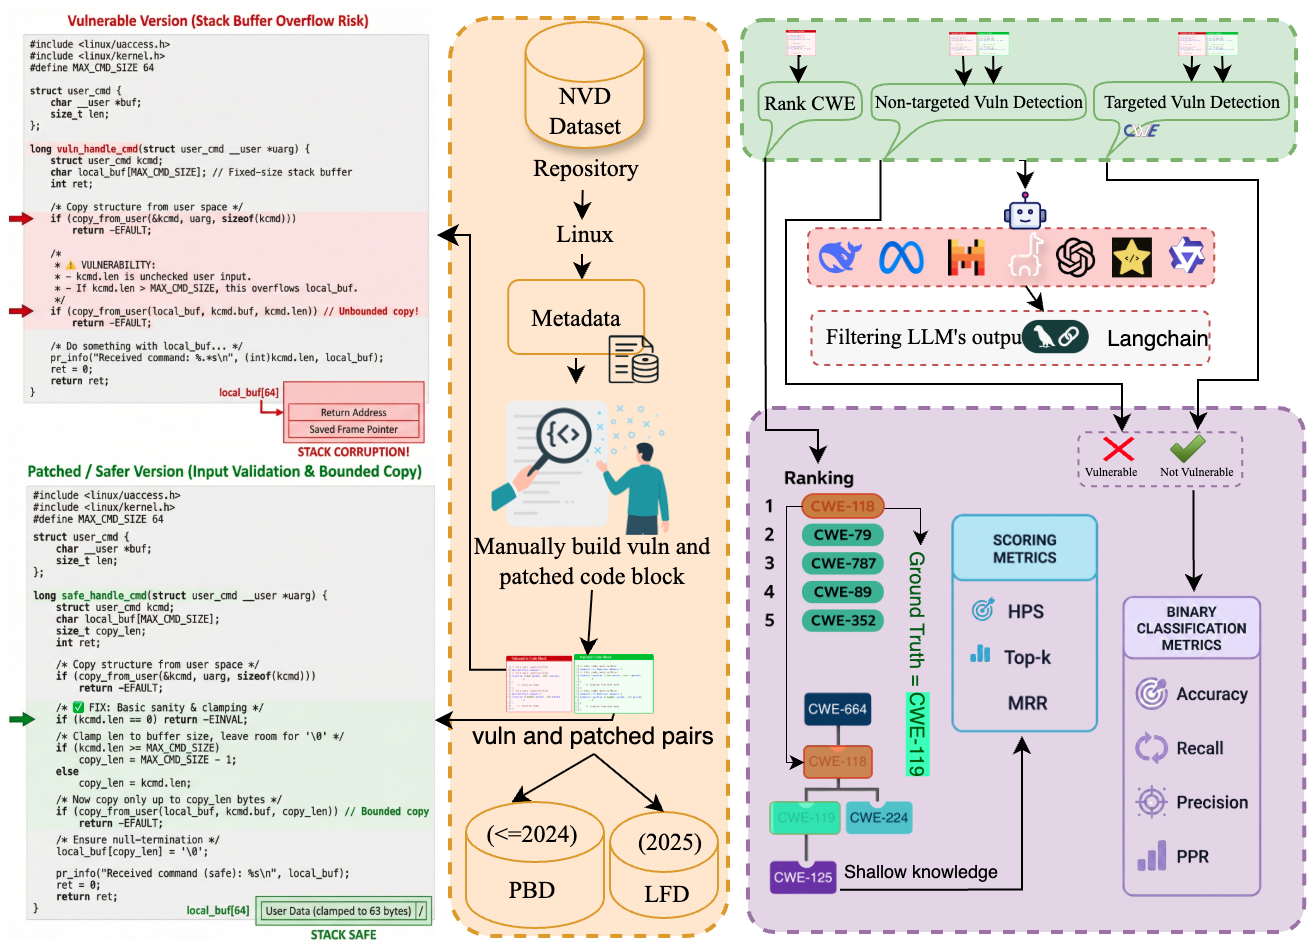
\includegraphics[width=1\textwidth]{figures/LLMKernelBench.png}}
		\caption{LLMKernelBench Framework. Metadata (commit messages, diffs, function/file names) and vulnerable-patched code pairs are extracted from Linux CVE commits. Prompts are designed for \gls{SVD} and CWE-label classification tasks in zero-shot settings. \glspl{LLM} perform detection and classification, while LangChain parses raw model outputs and a response audit separates binary verdicts, genuine abstentions, and invalid outputs}. Detection is evaluated using binary and ranking metrics.
	\label{figure:framework}
\end{figure*}
\section{Benchmarking Approach}
\label{section:approach}

LLMKernelBench is designed to assess pre-trained \glspl{LLM} (see Table~\ref{table:llm-specs} for the models evaluated) on \gls{SVD} and CWE-label classification tasks, focusing on C code from the Linux kernel while being extensible to other programming languages. As illustrated in Figure~\ref{figure:framework}, the framework is based on vulnerability metadata and code pairs extracted from Linux CVE commits, and includes prompts designed for \gls{SVD} and CWE-label classification tasks. Raw model outputs are processed through the LangChain \texttt{VulnerabilityOutputParser}; for response-validity analysis, we additionally audit the raw text to distinguish genuine uncertainty from malformed or otherwise non-compliant output. The primary open-source SVD evaluation uses temperature 0 for deterministic decoding. The response-validity sweep averages the two complete temperature-0.1 runs, including GPT-4.1-mini, whereas the CWE-ranking analysis averages its three available ranking runs. We use binary classification metrics (precision, recall, accuracy, F1) for \gls{SVD} and ranking metrics for CWE-label classification. This approach ensures benchmark reliability through representativeness (diverse real-world vulnerabilities), adaptability (an extendable methodology), portability (applicability across various \glspl{LLM}), and fairness (standardized evaluation procedures).
Section \ref{section:dataset} details our dataset construction process. Section \ref{section:metrics} defines metrics for both \gls{SVD} and CWE-label classification tasks. Finally, Section \ref{section:prompts} presents our standardized prompt templates.


\subsection{Dataset}
\label{section:dataset}
Our method systematically extracts pairs of vulnerable code blocks and their corresponding patched versions from real-world Linux kernel commits. We focus on the Linux kernel due to its rich vulnerability history and critical security importance. We collect commit hashes, CVE identifiers, and \gls{CWE} classifications from well-known vulnerability databases, including NVD~\cite{nvd2025}, in line with established practices~\cite{pereira2022software}. For each vulnerability-fixing commit, we retrieve the vulnerable code from its parent commit (pre-fix version) and the patched code from the commit itself (post-fix version).

Our extraction process identifies all security-related functions and non-functional elements (global variables, macros, type definitions, structs/unions, headers) that were directly modified in each commit. We include only functions with actual line-level changes, excluding unchanged code to avoid label noise. Non-functional elements are tracked separately as they often form critical vulnerability contexts that influence execution across multiple functions. This comprehensive approach assembles cohesive, vulnerable, and patched code blocks at multiple abstraction levels (single function, multiple functions, multiple files), enabling \glspl{LLM} to analyze complete contextual information rather than isolated fragments.

After extraction, the dataset is divided into two. The \gls{PBD} covers all vulnerabilities discovered on or before 2024, while the \gls{LFD} covers the more recent 2025 vulnerabilities. This division enables us to evaluate the impact of potential data leakage on the model's performance, thereby increasing our confidence in the generalizability of our findings.

\textbf{Manual Review, Denoising, and Deduplication.} Our automated extraction process allowed us to collect a total of 400 samples for PBD and 110 samples for LFD. After that, to ensure dataset integrity and label fidelity, both datasets were manually validated by two different reviewers. For this validation, a standardized protocol that defined inclusion criteria, exclusion criteria, and required evidence documentation was first defined. Then, the original datasets were split in half, and each half was assigned to a different reviewer. The reviewers followed the previously defined documentation to clean the dataset. Doubtful cases were marked for discussion and resolved through consensus sessions between the reviewers. The following validations were performed:

\begin{itemize}
    \item \textbf{Denoising}: Removed samples and functions/files where the changes were not security-related.
    \item \textbf{Completeness check}: Ensured all relevant and security-impacting changes from each commit were included.
    \item \textbf{\gls{CWE} frequency filtering}: CWEs that appeared only once were removed to improve representativeness.
    \item \textbf{Comment removal}: Stripped all code comments from both vulnerable and patched code blocks to eliminate potential biases and ensure that the \glspl{LLM} relied solely on code structure and semantics for \gls{SVD}.
    \item \textbf{Deduplication}: Removed duplicate or near-duplicate code samples (e.g., identical functions, commits, or cloned files) to prevent models from seeing the same or highly similar code during testing.
    \item \textbf{\gls{CWE} labeling}: In the LFD, 40 samples lacked \gls{CWE} identifiers in the NVD database; we manually labeled these samples, strictly adhering to NVD criteria for consistent labeling.
\end{itemize}

Table~\ref{table:dataset-stats} summarizes the overall size and composition of the \gls{PBD} and \gls{LFD} after this comprehensive cleaning process. The final \gls{PBD} dataset comprises 314 samples spanning 74 distinct CWEs, while the final \gls{LFD} dataset contains 103 samples belonging to 19 CWEs.

%The fundamental approach of LLMKernelBench assembles all touched functions and non-functional elements (macros, libraries, type definitions) into cohesive vulnerable and patched code blocks that \glspl{LLM} can comprehensively analyze for vulnerability prediction, ensuring complete contextual understanding rather than isolated code fragment analysis.

%Initially, we collected 400 samples for PBD and 110 samples for LFD through our automated extraction process. To ensure dataset integrity and label fidelity, both datasets underwent rigorous quality control through a structured two-author review process. Two authors independently evaluated every sample using a standardized protocol that defined inclusion criteria (security-relevant commits with confirmed CVE identifiers, function-level line modifications, and extractable vulnerable-patched pairs), exclusion criteria (cosmetic refactoring, formatting-only changes, test modifications, and commits lacking substantiated security relevance), and required evidence documentation (CVE/\gls{CWE} identifiers, commit metadata, and security rationale). Each reviewer assigned decision labels (Keep, Exclude, Requires-Discussion) with documented reasoning codes to ensure traceability and reproducibility. Inter-reviewer agreement was measured using Cohen's kappa, and all disagreements were resolved through consensus sessions with explicit rationale recording. Systematic denoising removed samples and touched functions/files that were not security-related, eliminating non-functional changes while preserving essential contextual elements necessary for semantic correctness. We removed singleton CWEs (vulnerabilities appearing only once) to ensure statistical reliability and prevent overrepresentation of rare, potentially outlier cases that could skew model evaluation. Additionally, we stripped all code comments from both vulnerable and patched code blocks to eliminate potential biases that could arise from human annotations, ensuring LLMs rely solely on code structure and semantics for VD. Deduplication removed duplicate or near-duplicate code samples (e.g., identical functions, commits, or cloned files) to prevent models from seeing the same or highly similar code during testing, employing both exact hash-based matching and token-level similarity metrics with manual inspection of flagged candidates to ensure canonical representation. Each dataset contained only one multi-label \gls{CWE} vulnerability, which we retained with comprehensive annotations rather than creating duplicate entries. For LFD, we manually labeled 40 samples that lacked \gls{CWE} identifiers in the NVD database, strictly adhering to NVD criteria for consistent labeling. After this comprehensive cleaning process, our final datasets comprised 314 samples in PBD and 103 samples in LFD. The fundamental approach of LLMKernelBench assembles all touched functions and non-functional elements (macros, libraries, type definitions) into cohesive vulnerable and patched code blocks that LLMs can comprehensively analyze for vulnerability prediction, ensuring complete contextual understanding rather than isolated code fragment analysis.

\textbf{\gls{CWE} Distribution and Label Space.} We did not pre-select a preferred subset of CWEs. PBD retains the CWE labels associated with the sampled Linux-kernel CVEs, while 40 LFD samples lacking NVD CWE identifiers were manually labeled under NVD-aligned criteria. The resulting label space, spanning 74 distinct CWEs in PBD and 19 in LFD, therefore reflects the sampled kernel vulnerabilities rather than an artificially balanced category design. Our dataset spans diverse \gls{CWE} categories organized according to the CWE-1000 hierarchical view \cite{cwe1000}. Table~\ref{table:cwe-pillars-combined} reports coverage against the ten fundamental \gls{CWE} pillars: eight have nonzero coverage in the sampled data, while deprecated or otherwise unmapped labels are grouped as CWE-OTHER. CWE-664 accounts for 43.3\% of PBD coverage, reflecting the prevalence of memory-related vulnerabilities in the Linux kernel. The distribution also includes 12.1\% deprecated \gls{CWE} identifiers (CWE-OTHER), representing historical vulnerability classifications that MITRE now marks as \enquote{PROHIBITED} for mapping.

\begin{table}[!t]
\centering
\caption{LLMKernelBench dataset statistics}
\label{table:dataset-stats}
\scriptsize
\setlength{\tabcolsep}{22pt}
\renewcommand{\arraystretch}{1.1}
\resizebox{\columnwidth}{!}{%
\begin{tabular}{@{}lrr@{}}
\toprule
\textbf{Metric} & \textbf{PBD} & \textbf{LFD} \\
\midrule
Vulnerabilities & 314 & 103 \\
Unique CWEs & 74 & 19 \\
\cmidrule(lr){1-3}
Files/Functions Changed (avg) & 1.5 / 2.0 & 1.1 / 1.3 \\
Vuln/Patched Lines (avg) & 109.4 / 114.1 & 60.9 / 63.6 \\
Lines Added/Deleted (avg) & 17.6 / 9.0 & 7.0 / 3.5 \\
\bottomrule
\end{tabular}
}
\end{table}




\begin{comment}
    \begin{table}[!t]
\centering
\caption{\gls{CWE} Pillar Distribution in PBD}
\label{table:cwe-pillars}
\renewcommand{\arraystretch}{1.1}
\small
\resizebox{\columnwidth}{!}{%
\begin{tabular}{@{}llcc@{}}
\toprule
\textbf{CWE-ID} & \textbf{Pillar Name} & \textbf{Coverage (\%)} \\
\midrule
CWE-664 & Improper Control of Resource Lifetime & 136 (43.3) \\
CWE-OTHER & Other/Unmapped CWEs & 12.1 \\
CWE-682 & Incorrect Calculation & 10.2 \\
CWE-284 & Improper Access Control & 8.9 \\
CWE-691 & Insufficient Control Flow Management & 8.6 \\
CWE-707 & Improper Neutralization & 5.7 \\
CWE-693 & Protection Mechanism Failure & 5.1 \\
CWE-710 & Improper Adherence to Coding Standards & 3.5 \\
CWE-703 & Improper Check/Handling of Except. Conditions & 2.9 \\
CWE-435 & Improper Interaction Between Components & 0.0 \\
CWE-697 & Incorrect Comparison & 0.0 \\
\bottomrule
\end{tabular}%
}
\vspace{-4pt}
\end{table}
\end{comment}





\begin{table}[!t]
\centering
\caption{\gls{CWE} pillar distribution across PBD and LFD.}
\label{table:cwe-pillars-combined}
\small
\renewcommand{\arraystretch}{1.1}
\resizebox{\columnwidth}{!}{%
\begin{tabular}{@{}llcc@{}}
\toprule
\textbf{CWE-ID} & \textbf{Pillar Name} & \multicolumn{2}{c}{\textbf{Coverage} (\%)} \\ 
\cmidrule(lr){3-4}
& & \textbf{PBD} & \textbf{LFD} \\
\midrule
CWE-664 & Improper Control of Resource Lifetime & 136 (43.3) & 62 (60.2) \\
CWE-OTHER & Other/Unmapped CWEs & 38 (12.1) & 0 (0.0) \\
CWE-682 & Incorrect Calculation & 32 (10.2) & 7 (6.8) \\
CWE-284 & Improper Access Control & 28 (8.9) & 0 (0.0) \\
CWE-691 & Insufficient Control Flow Management & 27 (8.6) & 11 (10.7) \\
CWE-707 & Improper Neutralization & 18 (5.7) & 9 (8.7) \\
CWE-693 & Protection Mechanism Failure & 16 (5.1) & 0 (0.0) \\
CWE-710 & Improper Adherence to Coding Standards & 11 (3.5) & 14 (13.6) \\
CWE-703 & Improper Check/Handling of Except. Conditions & 9 (2.9) & 0 (0.0) \\
CWE-435 & Improper Interaction Between Components & 0 (0.0) & 0 (0.0) \\
CWE-697 & Incorrect Comparison & 0 (0.0) & 0 (0.0) \\
\bottomrule
\end{tabular}%
}
\end{table}


\subsection{Tasks}
\label{section:tasks}

Based on this dataset, the models are evaluated across two different tasks: \gls{SVD} and vulnerability type identification.

\textbf{\gls{SVD}}. In this task, the models are given either a vulnerable code block (pre-fix versions from parent commits) or a non-vulnerable (patched) code block (post-fix versions from fixing commits). They are then asked to classify the code block as vulnerable (\texttt{1}), non-vulnerable (\texttt{0}), or to answer \texttt{not sure}. The uncertainty response is represented as $-1$ in the structured evaluation data. This third option is used because: (1) real-world \gls{SVD} often involves ambiguous cases where even security experts disagree; (2) it prevents \glspl{LLM} from making forced binary decisions when evidence is insufficient, potentially reducing false positives and negatives; and (3) it mirrors practical security analysis workflows where analysts may need to flag code for further investigation rather than making definitive vulnerability determinations. 

%It is important to note that, for all binary \gls{SVD}/\gls{SPV} tasks (SVD3--SVD6), we use labels $y\in\{1,0\}$, where $y=1$ denotes \emph{vulnerable} code (the pre-fix version from the parent commit) and $y=0$ denotes \emph{patched} code (the post-fix version from the fixing commit). During inference we allow models to abstain with $-1$ (\enquote{not sure}); this is an optional prediction class and \emph{not} a ground-truth label.

\textbf{CWE-label classification.} The \gls{CWE} taxonomy organizes weaknesses into a hierarchical structure with four abstraction levels as shown in Figure~\ref{fig:cwe_hierarchy}: \textit{Pillars} (highest level, 10 fundamental categories representing root security principles such as CWE-664 Improper Control of a Resource Through its Lifetime), \textit{Classes} (general weakness types like CWE-119 Buffer Errors), \textit{Bases} (specific weakness variants such as CWE-120 Buffer Copy without Checking Size of Input), and \textit{Variants} (detailed platform-specific manifestations). This hierarchy is formalized in the CWE-1000 Research Concepts view~\cite{cwe1000}.
% \begin{figure*}
%     \centering
%     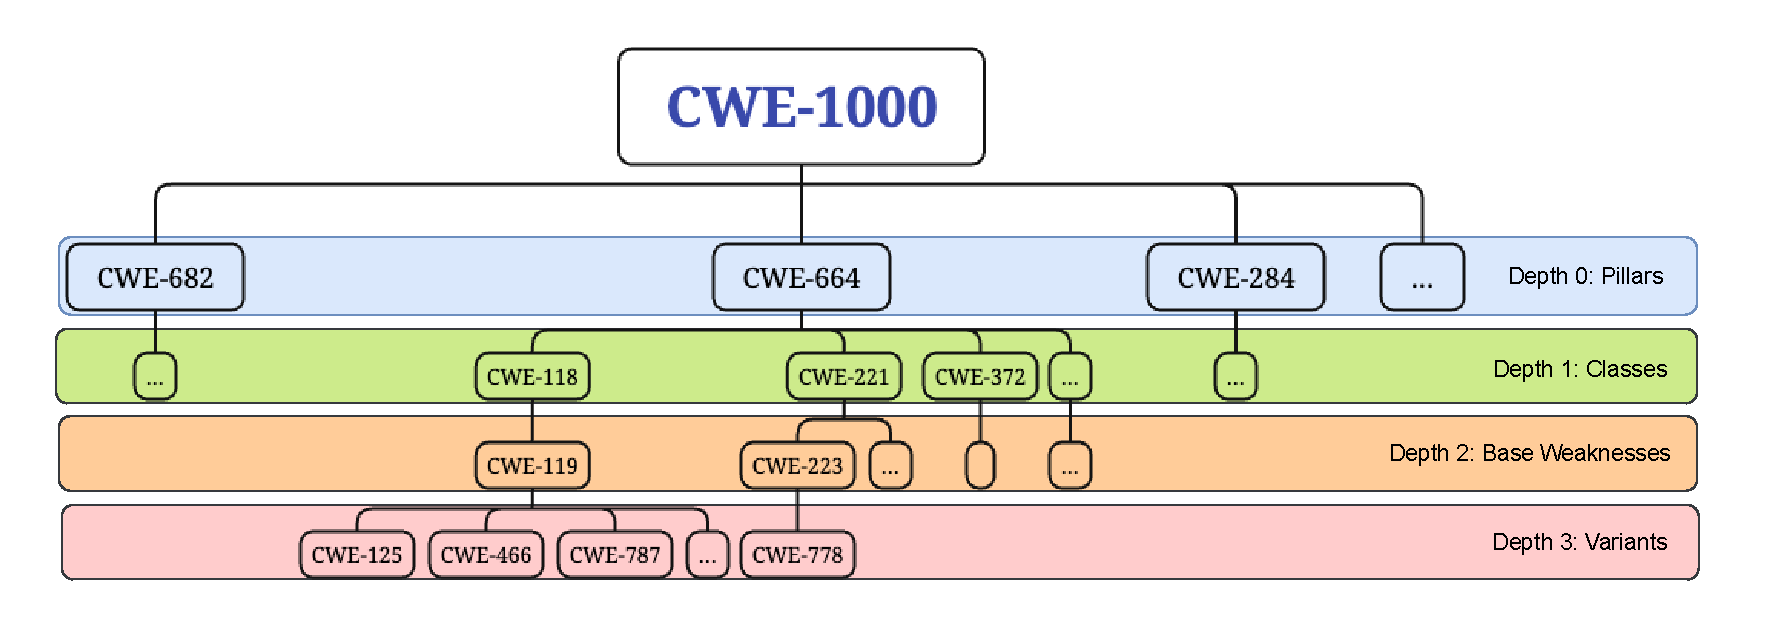
\includegraphics[width=0.8\textwidth]{figures/cwe_hierarchy.pdf}
%     \caption{CWE hierarchy}
%     \label{fig:cwe_hierarchy}
% \end{figure*}

\begin{figure}[h]
    \centering
    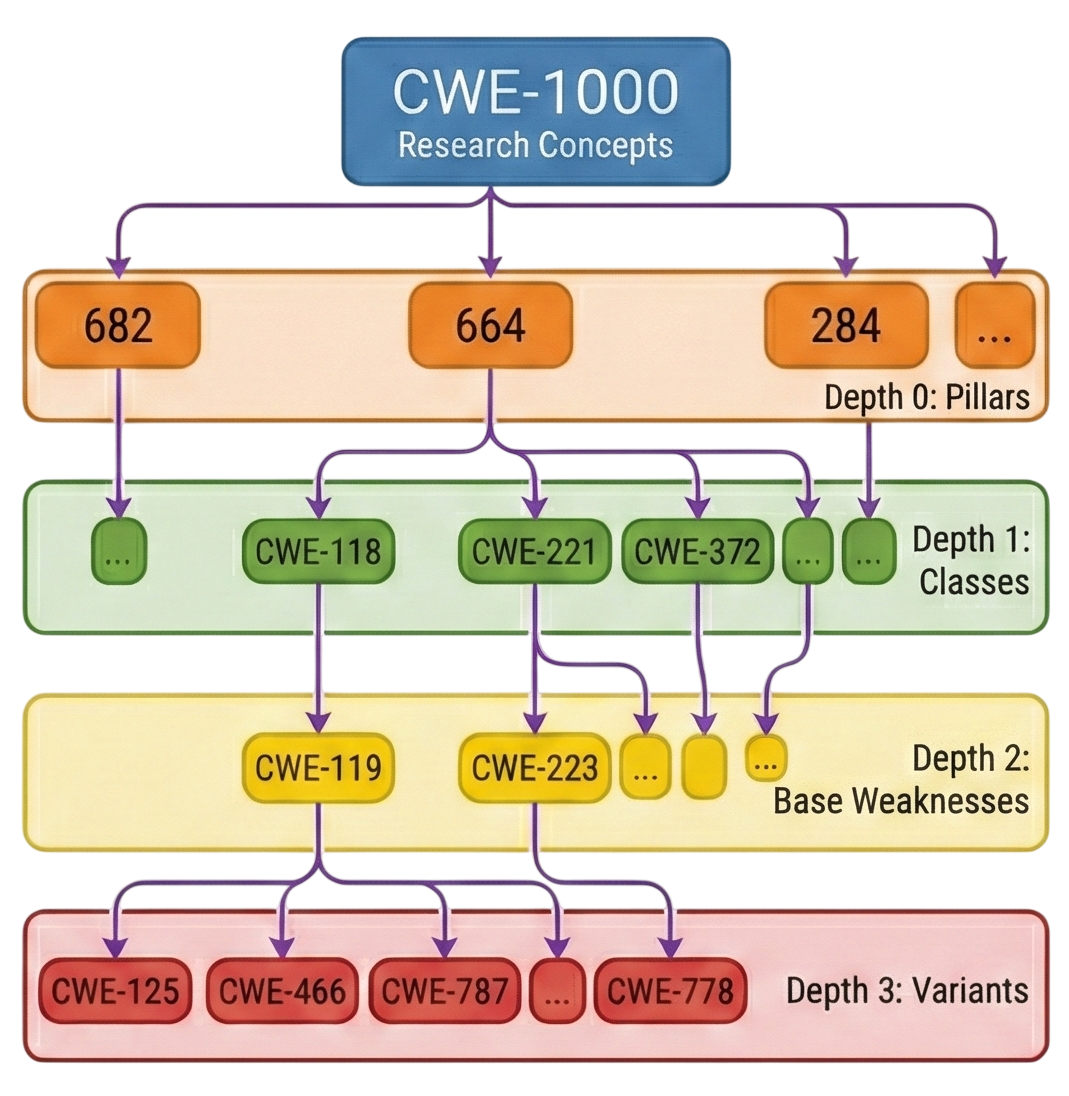
\includegraphics[width=0.8\columnwidth]{figures/cwe_hierarchy.png}
    \caption{CWE hierarchy.}
    \label{fig:cwe_hierarchy}
\end{figure}

For our \gls{CWE} classification tasks, we employ a \textit{hierarchical evaluation approach} that assesses model predictions across all taxonomy levels rather than focusing solely on exact matches.
This design measures the taxonomic proximity of model outputs, distinguishing broad category-level matches from exact fine-grained identification without assuming that proximity alone demonstrates semantic understanding.

We introduce the \gls{HPS} metric (\S\ref{section:metrics}), which assigns ordinal credit according to exact, immediate parent/child, sibling, same-root, or unrelated relations in the CWE-1000 hierarchy.
A prediction of CWE-121 (Stack-based Buffer Overflow) when the true answer is CWE-787 (Out-of-bounds Write) receives partial child credit, recording a related candidate despite missing the exact type.
This approach addresses practical challenges in \gls{CWE} classification: fine-grained labels (bases and variants) exhibit severe class imbalance, with many specific types having fewer than 10 examples in real-world datasets, rendering exact-match accuracy unreliable.
Meanwhile, coarse-grained evaluation at only the pillar level (10 categories) would be too lenient to distinguish precise weakness identification from broad category prediction.

Our hierarchical scoring thus separates exact Top-1 identification from taxonomically related candidate output. High HPS with low Top-1 accuracy indicates related labels in the candidate set, not necessarily taxonomy-aware reasoning.
This multi-level evaluation helps model developers locate error patterns and helps practitioners judge whether candidate labels are suitable only for routing or are accurate enough for diagnosis.

By considering both these tasks, our benchmark systematically evaluates \glspl{LLM} in terms of their ability to (1) detect the presence of vulnerabilities through binary \gls{SVD} classification, and (2) identify and prioritize the most likely underlying vulnerability types through \gls{CWE}-label ranking.

\subsection{Metrics}
\label{section:metrics}

Due to the different nature of the two tasks, different metrics must be employed. These metrics, along with statistical significance testing, are discussed next. 

\subsubsection{SVD}

To evaluate the models' performance at \gls{SVD}, we consider the following terms: \gls{TP} refers to the number of vulnerable code samples that the model correctly identifies as vulnerable; \gls{FP} is the number of non-vulnerable samples incorrectly predicted as vulnerable; \gls{TN} represents the number of non-vulnerable samples correctly classified as non-vulnerable; while \gls{FN} represents the number of vulnerable samples that the model fails to identify, incorrectly classifying them as non-vulnerable. These four quantities form the basis for calculating the performance metrics described below.

It is important to note that these metrics are computed only for cases in which the models provided a valid binary classification, i.e., vulnerable (\texttt{1}) or non-vulnerable (\texttt{0}). Genuine abstentions and invalid outputs are excluded. We distinguish these outcomes by auditing the raw response: a \emph{genuine abstention} clearly selects \texttt{not sure} (either alone or as an unambiguous final verdict motivated by insufficient information), whereas an \emph{invalid response} does not yield a single resolvable verdict, for example because it continues the input code, loops, or presents contradictory choices. Reporting these categories separately is critical because parser failure or prompt non-compliance should not be interpreted as model uncertainty. The following metrics are used:

\begin{itemize}
    \item \textbf{Accuracy}: measures the proportion of correctly classified code samples among all samples:

    \begin{equation}
    \text{Accuracy} = \frac{TP+TN}{TP+FP+TN+FN}
    \end{equation}
    
    As the dataset is relatively balanced between vulnerable and non-vulnerable samples, the accuracy accurately reflects the model’s overall performance without being dominated by one class. High accuracy is important as it indicates that the model performs well across both classes.
    
    \item \textbf{Recall} – measures the proportion of actual vulnerable code samples that were correctly identified by the model:
    
    \begin{equation}
        \text{Recall} = \frac{TP}{TP+FN}
    \end{equation}
    
    In this context, it represents the number of true vulnerabilities the \gls{LLM} successfully detects or flags. High recall is crucial, as missing vulnerable samples could lead to the overlooking of potential security issues.
    
    \item \textbf{Precision} – measures the proportion of code samples predicted as vulnerable that are truly vulnerable: 
    
    \begin{equation}
        \text{Precision} = \frac{TP}{TP+FP}
    \end{equation}
    
    This metric indicates how many of the flagged samples are genuine vulnerabilities rather than false positives. High precision is important to reduce the number of incorrect alerts, which can waste time during manual inspection or downstream analysis.
    
    \item \textbf{\gls{PPR}} – measures the proportion of all samples that the model classifies as vulnerable, regardless of correctness:
    
    \begin{equation}
    \text{PPR} = \frac{TP+FP}{TP+FP+TN+FN}
    \end{equation}
    
    While this metric is not as critical as precision or recall, it provides valuable insight into the model’s potential bias toward one class. A higher PPR may indicate a tendency to over-predict vulnerabilities, whereas a lower PPR suggests under-prediction. Comparing the PPR across models helps identify whether a model systematically favors one class over the other, offering additional context for interpreting performance results.

\end{itemize}

Together, these metrics provide a comprehensive evaluation of classification performance, balancing correctness, sensitivity, and class bias.

\subsubsection{CWE-label classification}
\label{section:cwe_metrics}
For the task of CWE-label classification, the following metrics are employed:

\begin{itemize}

	\item \textbf{Top-k Accuracy}~\cite{russakovsky2015imagenet}: Considers a prediction correct if the true vulnerability type appears among the model's k highest-ranked predictions. We measure Top-1 to Top-5 accuracy to evaluate how well models detect and rank both CVEs and CWEs. This progressive evaluation is particularly valuable in security contexts where identifying the correct vulnerability category among top candidates enables more efficient remediation efforts, even when exact classification is challenging.

	\item \textbf{\gls{MRR}}~\cite{craswell2009mean}: Evaluates ranking quality by calculating:
    
    \begin{equation}
        \frac{1}{N}\sum_{i=1}^{N}\frac{1}{\text{rank}_i}
    \end{equation}
    
    Where $\text{rank}_i$ is the position of the correct answer in the ranked list for the $i$-th query. MRR rewards models that rank the correct vulnerability type higher, recognizing that, in security contexts, prioritizing findings is crucial.

    \item \textbf{\gls{HPS}} scores a model's outputs by how close they are to the ground-truth \gls{CWE} in the hierarchy. We assign weights: $\text{exact}=1.0$, $\text{parent}=0.8$, $\text{child}=0.7$, $\text{sibling}=0.6$, $\text{same-root}=0.4$, $\text{unrelated}=0.0$. CWE-1000 is a directed acyclic graph rather than a strict tree because a weakness may have multiple parents or occur under multiple pillars. Parent and child therefore denote any immediate taxonomy edge, siblings share at least one immediate parent, and same-root labels share at least one top-level pillar. The HPS weighting scheme follows an ordinal decay aligned with the CWE hierarchy rather than modeling precise semantic distances. Higher weights reflect closer ancestry in the taxonomy, as confusing a vulnerability with an immediate parent or child category indicates greater taxonomic proximity than predicting an unrelated weakness. The specific values preserve hierarchical ordering and distinguish near-misses from unrelated predictions; they do not encode calibrated semantic margins. Formally, let $Y_i$ be the set of ground-truth labels and $(\hat y_{i1},\dots,\hat y_{ik_i})$ the valid predicted labels. Define $r(\hat y,y)\in\{\text{exact},\text{parent},\text{child},\text{sibling},\text{root},\text{none}\}$ and a weight map $w(\cdot)$ as above. Each predicted label receives its best score against the ground-truth set,
    
    \begin{equation}
      s_{ij}=\max_{y\in Y_i} w\big(r(\hat y_{ij},y)\big),
    \end{equation}
    
    and the implemented dataset score averages across all valid predicted labels,
    \begin{equation}
      \mathrm{HPS}=\frac{\sum_i\sum_{j=1}^{k_i}s_{ij}}{\sum_i k_i}.
    \end{equation}
    Thus HPS measures taxonomic proximity of the candidate set, while Top-$k$ accuracy and MRR separately measure exact inclusion and rank. For the supporting distance audit in Tables~\ref{tab:hps_validation_stats} and~\ref{tab:hierarchy_distance_dist}, distance is the shortest path in the undirected CWE-1000 parent--child graph. We connect the ten top-level pillars through a virtual root so that cross-pillar errors have finite distances; unmapped or deprecated identifiers remain unmeasurable. The committed HPS and distance-analysis scripts preserve all parent and pillar memberships and regenerate the reported values directly from the three ranking runs.

    To ground this metric in a practical security context, consider a true CWE-787 (Out-of-bounds Write) with a predicted CWE-121 (Stack-based Buffer Overflow). CWE-121 is an immediate child of CWE-787 in the benchmark hierarchy and therefore receives the child weight of 0.7. By contrast, CWE-284 (Improper Access Control) is in a different root branch and receives 0.0. In SOC triage, the former can still route an alert toward buffer-handling review, but it must not be treated as an exact diagnosis.
    
\end{itemize}

By combining these metrics, we evaluate classification accuracy, ranking quality, and the taxonomic proximity of predicted vulnerability categories.


\subsubsection{Statistical Significance Testing}
To assess whether performance differences are statistically meaningful rather than random, we combine group-level tests, degradation metrics, and correlation analysis.

\textbf{Statistical test selection.} To compare accuracy across abstraction levels (L1--L3), we first check normality (Shapiro-Wilk~\cite{shapiro1965analysis}) and homogeneity of variance (Levene). We then apply one-way ANOVA~\cite{fisher1970statistical} when both hold, Welch's ANOVA when variances differ, and the non-parametric Kruskal-Wallis H-test when normality fails. PBD satisfies both assumptions (Levene p=0.812), justifying ANOVA, whereas LFD Level~3 fails normality (p=0.008) and uses Kruskal-Wallis; p$<$0.05 denotes a significant effect of abstraction level on accuracy.

\textbf{Degradation} quantifies robustness to context as $\text{Accuracy}_{\text{L1}}-\text{Accuracy}_{\text{L3}}$: positive values denote decline with broader scope, negative values improvement, and near-zero values stable behavior across levels.

\textbf{Pearson correlation} ($r\in[-1,1]$) measures the strength and direction of the linear relationship between two continuous variables (e.g., context window size vs.\ degradation), with significance assessed via its p-value.

\textbf{Mann-Whitney U}~\cite{mann1947test} is a non-parametric, rank-based test for two independent groups that is robust to outliers and skewed or unequal-sized samples. We use it to compare Simple (L1) versus Complex (L2+L3) accuracy in LFD, where the small L3 sample (n=3) and group imbalance (85 vs.\ 18) violate parametric assumptions. We pair it with the \textbf{rank-biserial correlation}~\cite{kerby2014simple} effect size,
\begin{equation}
    r = 1 - \frac{2U}{n_1 \cdot n_2},
\end{equation}
where $U$ is the Mann-Whitney statistic and $n_1,n_2$ the group sizes, to report practical magnitude alongside significance using Cohen's thresholds~\cite{cohen1988statistical} (negligible $|r|<$0.1, small, medium, large $|r|\geq$0.5). This matters under strong imbalance, where small differences can reach significance from sample size alone.

\subsection{Prompt Templates}
\label{section:prompts}

\begin{figure}[!t]
\centering
\fbox{\begin{minipage}{0.94\columnwidth}
\ttfamily\footnotesize
Check if the following C code block is vulnerable.\\
Respond with ONLY one of these options:\\
- '1' if the code is vulnerable\\
- '0' if the code is not vulnerable\\
- 'not sure' if you are not sure if it is vulnerable or not\\[2pt]
Do not include any explanation or additional text.\\[2pt]
Code block:\\
\{code\}\\[2pt]
Response:
\end{minipage}}
	\caption{Verbatim vulnerability-detection template used in the production pipeline; patch verification substitutes the patched code block.}
	\label{figure:prompt_svd3}
\end{figure}
\begin{figure}[!t]
\centerline{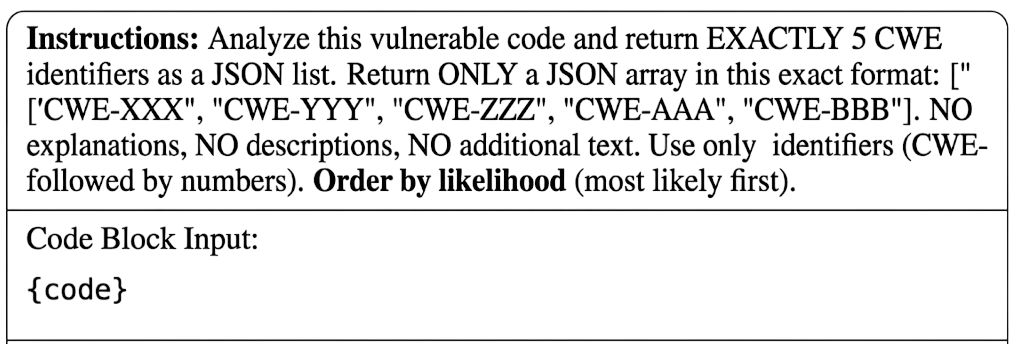
\includegraphics[width=1.0\columnwidth]{figures/promptSVD2.png}}
	\caption{\gls{CWE} ranking prompt.}
	\label{figure:prompt_svd2}
\end{figure}

Our prompt templates for both \gls{SVD} and CWE-label classification are designed with four key principles in mind: clear task specification, structured output formats, minimal introduction of bias, and scalability across vulnerability types. We focus on benchmarking the inherent \gls{LLM} capabilities rather than optimizing prompting strategies, and on evaluating baseline performance to inform future research directions. As shown in Figure~\ref{figure:prompt_svd3}, each prompt clearly states the expected task and output format, including explicit three-way response instructions (\texttt{1}, \texttt{0}, or \texttt{not sure}; the uncertainty response is stored as \texttt{-1} for evaluation), uses standardized templates for fair comparison across models, maintains essential code context while avoiding information leakage, and reflects real-world security analysis scenarios.

Representative prompt formats are shown in Figures~\ref{figure:prompt_svd3} (\gls{SVD}) and~\ref{figure:prompt_svd2} (CWE-label classification).

%\begin{table}[h!]
%\centering
%\captionsetup{skip=2pt,font=small}
%\caption{Prompt Templates for SVD and \gls{SPV} Tasks}
%\label{table:prompt_templates}
%\setlength{\tabcolsep}{1.5pt}
%\renewcommand{\arraystretch}{0.9}
%{\scriptsize
%\begin{tabularx}{\columnwidth}{@{\extracolsep{\fill}}%
%l l
%>{\centering\arraybackslash}p{0.053\columnwidth}%
%>{\centering\arraybackslash}p{0.053\columnwidth}%
%>{\centering\arraybackslash}p{0.060\columnwidth}%
%>{\centering\arraybackslash}p{0.060\columnwidth}%
%X@{}}
%\toprule
%\multicolumn{1}{c}{\textbf{ID}} &
%\multicolumn{1}{c}{\textbf{Task}} &
%\multicolumn{4}{c}{\textbf{Inputs}} &
%\multicolumn{1}{c}{\textbf{Description}} \\
%\cmidrule(lr){3-6}
%& & \multicolumn{1}{c}{\textbf{V}} &
%\multicolumn{1}{c}{\textbf{P}} &
%\multicolumn{1}{c}{\textbf{CVE}} &
%\multicolumn{1}{c}{\textbf{CWE}} & \\
%\midrule
%SVD2 & \gls{CWE} Ranking  & Y  & -- & -- & -- & Rank top-5 CWEs for given code. \\
%SVD3 & Detection    & Y  & -- & -- & -- & Detect whether code is vulnerable (non-targeted). \\
%SVD4 & Verification & -- & Y  & -- & -- & Verify patched code is safe (non-targeted). \\
%SVD5 & Detection    & Y  & -- & Y  & Y  & Detect vulnerability for a specific CVE/\gls{CWE} (targeted). \\
%SVD6 & Verification & -- & Y  & Y  & Y  & Verify patch for a specific CVE/\gls{CWE} (targeted). \\
%\bottomrule
%\end{tabularx}
%}
%\vspace{2pt}
%\raggedright\scriptsize
%V: vulnerable code (pre-fix); P: patched code (post-fix). All tasks use zero-shot prompts.
%\end{table}



\section{Benchmarking Results}
\label{section:results}

In this study, we leverage seven pre-trained \glspl{LLM} to assess their capabilities in \gls{SVD} and CWE-label classification tasks. Our selection comprises three code-specialized models (CodeLlama~\cite{roziere2023code}, StarCoder2 \cite{lozhkov2024starcoder}, and Qwen3-Coder~\cite{yang2025qwen3}) explicitly trained on programming repositories, and four general-purpose models (Llama3.1~\cite{dubey2024llama}, Mistral~\cite{jiang2023mistral7b}, and DeepSeek-R1~\cite{guo2025deepseek}, GPT-4.1-mini~\cite{openai2025gpt4_1mini}) designed for broader language understanding tasks. This balanced selection enables us to investigate whether domain-specific training provides advantages over general language comprehension for security-critical tasks. We selected these models based on five key criteria: (1) their state-of-the-art performance on code understanding and generation benchmarks, (2) architectural diversity spanning both standard fully-dense models (e.g., CodeLlama) and \gls{MoE} models (e.g., DeepSeek-R1) to ensure comprehensive evaluation, (3) varying parameter sizes (7B-30B and unknown for GPT-4.1-mini) and context window capacities (16K-1M tokens) to investigate how model scale and memory affect \gls{SVD} capabilities, (4) balanced representation of code-specialized versus general-purpose training to assess domain expertise effects, and (5) inclusion of both smaller open-source and larger proprietary models, allowing for a fair comparison across accessibility and capability dimensions. The specifications of the models we used are detailed in Table~\ref{table:llm-specs}.

\begin{table}[!t]
\centering
\caption{LLM specs with context window sizes (tokens).}
\label{table:llm-specs}
\footnotesize
\setlength{\tabcolsep}{6pt}
\renewcommand{\arraystretch}{1.1}
\begin{tabular}{@{}l l r r@{}}
\toprule
\textbf{Model} & \textbf{Type} & \textbf{\# Params} & \textbf{Context Window} \\
\midrule
CodeLlama & Code-spec. & 7B & 16K \\
StarCoder2 & Code-spec. & 7B & 16K \\
Qwen3-Coder & Code-spec. & 30B & 262K \\
Llama3.1 & General & 8B & 131K \\
Mistral (v0.3) & General & 7B & 32K \\
DeepSeek-R1 & General & 7B & 131K \\
GPT-4.1-mini & General & --- & 1M \\
\bottomrule
\end{tabular}
\end{table}

\subsection{RQ1: Overall \gls{SVD} performance}
\label{section:rq1}

For this research question, we first separate valid binary verdicts from genuine abstentions and invalid outputs. We then analyze classification performance in two settings: non-targeted, where no specific CWE is provided, and targeted, where the prompt includes the CWE label. Because the validated response rates supplied for this audit are pooled over both settings and both datasets, Table~\ref{tab:abst-model-non-targeted} reports the overall temperature-0 response distribution rather than unsupported setting-specific estimates. Each available model contributes 1,668 responses (417 vulnerable/patched pairs evaluated in both settings).

\begin{table}[h]
\centering%\color{red}
\caption{Response validity at temperature 0, pooled over non-targeted/targeted settings and PBD/LFD. \emph{Valid}: a resolvable 0/1 verdict; \emph{Genuine abstention}: a clear uncertainty verdict; \emph{Invalid}: non-compliant or indeterminate output. GPT-4.1-mini was not run at this temperature.}
\label{tab:abst-model-non-targeted}
\begin{tabular}{lrrr}
\hline
\textbf{Model} & \textbf{Valid (\%)} & \textbf{Genuine abst.\ (\%)} & \textbf{Invalid (\%)} \\
\hline
CodeLlama       & 98.20 & 0.00 & 1.80 \\
DeepSeek-R1     & 100.00 & 0.00 & 0.00 \\
GPT-4.1-mini    & -- & -- & -- \\
Llama3.1        & 100.00 & 0.00 & 0.00 \\
Mistral         & 98.62 & 0.00 & 1.38 \\
Qwen3-Coder-30B & 99.46 & 0.06 & 0.48 \\
StarCoder2      & 73.92 & 0.00 & 26.08 \\
\hline
\end{tabular}
\end{table}

\textbf{Genuine abstention is rare, while most non-answers are formatting failures.}
At temperature 0, Qwen3-Coder is the only model with observed genuine abstentions (0.06\%). The other open-source models have no genuine abstentions. Invalid output is below 2\% for CodeLlama, Mistral, and Qwen3-Coder, and absent for DeepSeek-R1 and Llama3.1. StarCoder2 is the clear exception: 26.08\% of its outputs are invalid, primarily because the base completion model continues code or otherwise fails to emit one of the requested verdicts. The broader decoding sweep in Table~\ref{tab:abst-temp} confirms that genuine abstention and invalid output are distinct behaviors: GPT-4.1-mini averages 2.40\% genuine abstention across the two temperature-0.1 runs, while StarCoder2's invalid rate reaches 26.08\% at temperature 0.

\subsubsection{Non-targeted Classification}
\label{section:rq1-nontargeted}

\textbf{\glspl{LLM} performed no better than random classifiers.} Table~\ref{tab:metrics-svd} presents the performance metrics for the cases where the models provided a classification. All models exhibit accuracies close to 50\%, irrespective of architecture, size, or context window size. This behaviour is observed on both \gls{PBD} and \gls{LFD}; the historical split does not show a clear aggregate advantage over the post-cutoff split. Because the splits differ in composition and size, this comparison constrains but does not isolate the causal effect of training-data exposure.

Consider CVE-2024-26599 (CWE-119, PBD), a clear out-of-bounds array access in a PWM driver function (Figure~\ref{figure:cve_2024_26599}). The vulnerable code validates that \texttt{args->args\_count} is either 1 or 2, but subsequently accesses \texttt{args->args[2]} when \texttt{args\_count == 2}. Since arrays are zero-indexed, valid indices are only 0 and 1, making this an obvious out-of-bounds access. The patch simply replaces \texttt{args[2]} with \texttt{args[1]}. A human reviewer can immediately identify this as vulnerable because it violates a basic array bounds constraint. Yet the models still struggled to distinguish the vulnerable and patched versions reliably. In the first run, GPT-4.1-mini correctly classified both the vulnerable and patched samples. CodeLlama, Mistral, and DeepSeek classified both as vulnerable, while Llama3.1 classified both as safe. StarCoder2 produced an invalid response for the vulnerable version and classified the patched version as safe. This example is consistent with the aggregate class biases in Table~\ref{tab:metrics-svd}: even when the local defect is explicit, several models preserve the same verdict across the vulnerable--patched pair rather than responding to the changed array index.

These results stand in sharp contrast to supervised detection tools evaluated under different assumptions: SecureFalcon~\cite{ferrag2025securefalcon} reports 94\% binary accuracy on C/C++ code after training on FormAI/FalconVulnDB, and Alam et al.\ report 99\% Solidity vulnerability-detection accuracy after fine-tuning GPT-3.5 Turbo and GPT-4o Mini~\cite{alam2024detection}. These figures are not directly comparable because the studies use task-specific training datasets and different software domains, whereas our evaluation measures zero-shot, off-the-shelf performance and includes a post-cutoff split.

\begin{figure}[!t]

\begin{lstlisting}[language=Diff, basicstyle=\scriptsize\ttfamily, xleftmargin=0pt, frame=single]
// File: drivers/pwm/core.c
of_pwm_single_xlate(struct pwm_chip *chip,
                    const struct of_phandle_args *args) {
    struct pwm_device *pwm;

    if (chip->of_pwm_n_cells < 1)
        return ERR_PTR(-EINVAL);

    // Validates that args_count is either 1 or 2
    if (args->args_count != 1 && args->args_count != 2)
        return ERR_PTR(-EINVAL);

    pwm = pwm_request_from_chip(chip, 0, NULL);
    if (IS_ERR(pwm))
        return pwm;

    pwm->args.period = args->args[0];
    pwm->args.polarity = PWM_POLARITY_NORMAL;

    // BUG: Accessing index 2 when count==2 (valid: 0,1)
-   if (args->args_count == 2 && args->args[2] & PWM_POLARITY_INVERTED)
+   if (args->args_count == 2 && args->args[1] & PWM_POLARITY_INVERTED)
        pwm->args.polarity = PWM_POLARITY_INVERSED;

    return pwm;
}
\end{lstlisting}

\caption{CVE-2024-26599: out-of-bounds access; patch shown.}
\label{figure:cve_2024_26599}
\end{figure}

\textbf{Models exhibit strong and consistent class biases rather than meaningful vulnerability detection behaviour.} Examining Recall, Precision, and \gls{PPR} reveals clear patterns across both datasets. In the non-targeted setting, CodeLlama, DeepSeek, Mistral, and Qwen3-Coder all achieve very high recall values (roughly 70--85\%) together with high \gls{PPR} values, indicating a strong tendency to classify most samples as vulnerable. However, their precision remains close to 50\%, showing that these high recall scores are largely driven by overpredicting the positive class rather than correctly identifying vulnerabilities. In contrast, GPT-4.1-mini and Llama3.1 exhibit the opposite behaviour, with low recall and low \gls{PPR} values across both datasets, indicating a strong bias toward predicting samples as non-vulnerable. Despite this conservative tendency, precision also remains close to random, meaning that even its positive predictions are unreliable. StarCoder2 appears comparatively more balanced, with recall and \gls{PPR} values closer to 50\%, but its overall accuracy still remains at chance level.


\begin{table*}[!t]
    %\color{red}
    \centering
    \caption{Performance metrics for \gls{SVD} in non-targeted and targeted settings.}
    \label{tab:metrics-svd}
    \scriptsize
    \renewcommand{\arraystretch}{1.0}
    %\setlength{\tabcolsep}{1.8pt}
    \begin{tabular}{l rr rr rr rr rr rr rr rr}
    \toprule
    \multirow{3}{*}{Model}
      & \multicolumn{8}{c}{\textbf{Non-Targeted}}
      & \multicolumn{8}{c}{\textbf{Targeted}} \\
    \cmidrule(lr){2-9} \cmidrule(lr){10-17}
      & \multicolumn{4}{c}{PBD (\%)} & \multicolumn{4}{c}{LFD (\%)}
      & \multicolumn{4}{c}{PBD (\%)} & \multicolumn{4}{c}{LFD (\%)} \\
    \cmidrule(lr){2-5} \cmidrule(lr){6-9} \cmidrule(lr){10-13} \cmidrule(lr){14-17}
      & Acc. & Rec. & Prec. & PPR 
      & Acc. & Rec. & Prec. & PPR 
      & Acc. & Rec. & Prec. & PPR 
      & Acc. & Rec. & Prec. & PPR \\
    \midrule
    CodeLlama & 49.9 & 73.3 & 49.9 & 73.5 & 50.5 & 69.9	& 50.3 & 69.4 & 51.7 & 88.2 & 51.0 & 86.6 & 52.9 & 90.0 & 51.7 & 87.1 \\
    DeepSeek & 49.6 & 81.3 & 50.1 & 80.1 & 50.0 & 77.7 & 50.0 & 77.7 & 49.6 & 87.3 & 50.2 & 86.1 & 51.9 & 86.4 & 51.3 & 84.5 \\
    GPT-4.1-mini & 50.8 & 5.2 & 59.9 & 4.4 & 51.5 & 5.5 & 70.0 & 4.0 & 49.6 & 7.4 & 47.3 & 7.9 & 52.6 & 8.4 & 72.6 & 5.8 \\
    Llama3.1 & 50.1 & 31.6 & 50.1 & 31.5 & 51.0 & 29.4 & 51.6 & 28.5 & 49.4 & 27.3 & 48.9 & 27.9 & 47.7 & 15.5 & 43.6 & 17.8 \\
    Mistral & 49.4 & 85.2 & 49.7 & 85.8 & 50.5 & 79.9 & 50.3 & 79.4 & 47.7 & 19.6 & 45.0 & 21.8 & 49.5 & 14.2 & 48.6 & 14.7 \\
    Qwen3-Coder & 50.3 & 84.6 & 50.3 & 84.4 & 49.0 & 79.6 & 49.4 & 80.6 & 50.0& 61.6 & 50.2 & 61.6 & 52.7 & 49.3 & 52.9 & 46.7 \\
    StarCoder2 & 49.0 & 52.2 & 47.0 & 52.7 & 49.9 & 48.8 & 49.5 & 49.3 & 49.2& 61.4 & 48.4 & 62.2 & 53.6 & 67.0 & 50.8 & 62.9 \\
    \bottomrule
    \end{tabular}
\end{table*}


\subsubsection{Targeted Classification}
\label{section:rq1-targeted}

\textbf{Providing the CWE label shifts model biases but does not improve classification performance.}
In the targeted setting, Table~\ref{tab:metrics-svd} (Targeted columns) summarizes the performance metrics. Accuracy remained near 50\% for all models, so providing the CWE label did not produce a clear aggregate improvement. However, examining recall and \gls{PPR} reveals notable bias shifts. CodeLlama and DeepSeek saw their positive class bias further amplified, with recall rising to around 88\% and 87\% on PBD respectively, while precision remained near 50\%. Mistral exhibited the most dramatic reversal, flipping from a strong positive bias (recall: 85.2\%) to a strong negative one (recall: 19.6\%). Llama3.1's existing negative bias deepened further, while Qwen3-Coder moved toward balance, with recall dropping from 84.6\% to 61.6\% on PBD. StarCoder2 and GPT-4.1-mini showed a modest increase in positive bias. Thus, CWE labels shift models in distinct and sometimes opposing directions without a consistent accuracy gain.

% \begin{table*}[!t]
%     \centering
%     \caption{Per-CWE breakdown of the performance metrics for \gls{SVD}.}
%     \label{tab:cwe-metrics-svd}
%     \scriptsize
%     \renewcommand{\arraystretch}{1.0}
%     %\setlength{\tabcolsep}{1.8pt}
%     \begin{tabular}{l rr rr rr rr rr rr rr rr}
%     \toprule
%     \multirow{3}{*}{CWE Pillar}
%       & \multicolumn{8}{c}{\textbf{Non-Targeted}}
%       & \multicolumn{8}{c}{\textbf{Targeted}} \\
%     \cmidrule(lr){2-9} \cmidrule(lr){10-17}
%       & \multicolumn{4}{c}{PBD (\%)} & \multicolumn{4}{c}{LFD (\%)}
%       & \multicolumn{4}{c}{PBD (\%)} & \multicolumn{4}{c}{LFD (\%)} \\
%     \cmidrule(lr){2-5} \cmidrule(lr){6-9} \cmidrule(lr){10-13} \cmidrule(lr){14-17}
%       & Acc. & Rec. & Prec. & PPR 
%       & Acc. & Rec. & Prec. & PPR 
%       & Acc. & Rec. & Prec. & PPR 
%       & Acc. & Rec. & Prec. & PPR \\
%     \midrule
%     CWE-284 & 50.0 & 38.7 & 52.2 & 38.3 & -- & -- & -- & -- & 45.0 & 32.3 & 45.5 & 36.7 & -- & -- & -- & -- \\
%     CWE-664 & 47.9 & 48.0 & 50.0 & 50.0 & 48.9 & 30.2 & 45.2 & 32.1 & 51.3 & 35.1 & 50.0 & 34.2 & 55.0 & 33.3 & 55.3 & 29.0 \\
%     CWE-682 & 54.1 & 51.5 & 58.6 & 47.5 & 40.0 & 33.3 & 50.0 & 40.0 & 44.3 & 27.3 & 47.4 & 31.1 & 40.0 & 16.7 & 50.0 & 20.0 \\
%     CWE-691 & 46.2 & 28.6 & 50.0 & 30.8 & 44.4 & 0.0 & 0.0 & 0.0 & 53.8 & 35.7 & 62.5 & 30.8 & 44.4 & 20.0 & 50.0 & 22.2 \\
%     CWE-693 & 54.2 & 47.6 & 47.6 & 43.8 & -- & -- & -- & -- & 58.3 & 47.6 & 52.6 & 39.6 & -- & -- & -- & -- \\
%     CWE-703 & 49.1 & 46.4 & 48.1 & 47.4 & -- & -- & -- & -- & 47.4 & 39.3 & 45.8 & 42.1 & -- & -- & -- & -- \\
%     CWE-707 & 43.1 & 42.3 & 44.0 & 49.0 & 56.1 & 40.9 & 64.3 & 34.1 & 43.1 & 38.5 & 43.5 & 45.1 & 51.2 & 31.8 & 58.3 & 29.3 \\
%     CWE-710 & 55.2 & 38.5 & 50.0 & 34.5 & 51.7 & 40.0 & 54.5 & 37.9 & 56.9 & 42.3 & 52.4 & 36.2 & 48.3 & 33.3 & 50.0 & 34.5 \\
%     CWE-OTHER & 49.0 & 38.2 & 49.1 & 39.5 & -- & -- & -- & -- & 49.1 & 38.8 & 49.0 & 40.2 & -- & -- & -- & -- \\
%     \bottomrule
%     \end{tabular}
% \end{table*}


\subsection{RQ2: Consistency across CWEs pillars}
\label{section:rq2}

\textbf{\glspl{LLM} show weak, near-chance performance across CWE pillars, reinforcing that they are not yet capable of reliable \gls{SVD} classification.}
In the non-targeted setting, performance varies slightly by pillar but remains close to random guessing. For \gls{PBD}, accuracies range from 48.3\% (CWE-OTHER) to 52.7\% (CWE-693), with most pillars clustered near 50\%. For \gls{LFD}, results are only available for a subset of pillars (CWE-664/682/691/707/710) and accuracies range from 49.3\% to 54.9\%. Beyond accuracy, the other metrics show the same overall weakness: in \gls{PBD}, recall spans 55.2\%--60.5\% and precision ranges from 48.7\% to 51.8\%. 

The same trends can be seen for \gls{LFD} and for the targeted setting, with models always remaining near chance across pillars, as summarized in Table~\ref{tab:cwe-metrics-svd}.

% \begin{table}[!t]
%     \centering
%     \caption{Per-CWE breakdown of the performance metrics for \gls{SVD}.}
%     \label{tab:cwe-metrics-svd}
%     \small
%     \renewcommand{\arraystretch}{1.0}
%     \setlength{\tabcolsep}{1.8pt}
%     \resizebox{\columnwidth}{!}{%
%     \begin{tabular}{lrrrrrrrrrr}
%     \toprule
%     \multirow{2}{*}{CWE Pillar} & \multicolumn{4}{c}{PBD (\%)} & \multicolumn{4}{c}{LFD (\%)} \\
%     \cmidrule(lr){2-5} \cmidrule(lr){6-9}
%     & \textbf{Acc.} & \textbf{Rec.} & \textbf{Prec.} & \textbf{PPR} & \textbf{Acc.} & \textbf{Rec.} & \textbf{Prec.} & \textbf{PPR} \\
%     \midrule
%     \multicolumn{9}{c}{\textit{Non-Targeted}} \\
%     \midrule
%     CWE-284 & 50.0 & 38.7 & 52.2 & 38.3 & - & - & - & - \\
%     CWE-664 & 47.9 & 48.0 & 50.0 & 50.0 & 48.9 & 30.2 & 45.2 & 32.1 \\
%     CWE-682 & 54.1 & 51.5 & 58.6 & 47.5 & 40.0 & 33.3 & 50.0 & 40.0 \\
%     CWE-691 & 46.2 & 28.6 & 50.0 & 30.8 & 44.4 & 0.0 & 0.0 & 0.0 \\
%     CWE-693 & 54.2 & 47.6 & 47.6 & 43.8 & - & - & - & - \\
%     CWE-703 & 49.1 & 46.4 & 48.1 & 47.4 & - & - & - & - \\
%     CWE-707 & 43.1 & 42.3 & 44.0 & 49.0 & 56.1 & 40.9 & 64.3 & 34.1 \\
%     CWE-710 & 55.2 & 38.5 & 50.0 & 34.5 & 51.7 & 40.0 & 54.5 & 37.9 \\
%     CWE-OTHER & 49.0 & 38.2 & 49.1 & 39.5 & - & - & - & - \\
%     \midrule
%     \multicolumn{9}{c}{\textit{Targeted}} \\
%     \midrule
%     CWE-284 & 45.0 & 32.3 & 45.5 & 36.7 & - & - & - & - \\
%     CWE-664 & 51.3 & 35.1 & 50.0 & 34.2 & 55.0 & 33.3 & 55.3 & 29.0 \\
%     CWE-682 & 44.3 & 27.3 & 47.4 & 31.1 & 40.0 & 16.7 & 50.0 & 20.0 \\
%     CWE-691 & 53.8 & 35.7 & 62.5 & 30.8 & 44.4 & 20.0 & 50.0 & 22.2 \\
%     CWE-693 & 58.3 & 47.6 & 52.6 & 39.6 & - & - & - & - \\
%     CWE-703 & 47.4 & 39.3 & 45.8 & 42.1 & - & - & - & - \\
%     CWE-707 & 43.1 & 38.5 & 43.5 & 45.1 & 51.2 & 31.8 & 58.3 & 29.3 \\
%     CWE-710 & 56.9 & 42.3 & 52.4 & 36.2 & 48.3 & 33.3 & 50.0 & 34.5 \\
%     CWE-OTHER & 49.1 & 38.8 & 49.0 & 40.2 & - & - & - & - \\
%     \bottomrule
%     \end{tabular}
%     }
% \end{table}

\begin{table*}[!t]
    \centering%\color{blue}
    \caption{Per-CWE breakdown of the performance metrics for \gls{SVD}.}
    \label{tab:cwe-metrics-svd}
    \scriptsize
    \renewcommand{\arraystretch}{1.0}
    %\setlength{\tabcolsep}{1.8pt}
    \begin{tabular}{l rr rr rr rr rr rr rr rr}
    \toprule
    \multirow{3}{*}{CWE Pillar}
      & \multicolumn{8}{c}{\textbf{Non-Targeted}}
      & \multicolumn{8}{c}{\textbf{Targeted}} \\
    \cmidrule(lr){2-9} \cmidrule(lr){10-17}
      & \multicolumn{4}{c}{PBD (\%)} & \multicolumn{4}{c}{LFD (\%)}
      & \multicolumn{4}{c}{PBD (\%)} & \multicolumn{4}{c}{LFD (\%)} \\
    \cmidrule(lr){2-5} \cmidrule(lr){6-9} \cmidrule(lr){10-13} \cmidrule(lr){14-17}
      & Acc. & Rec. & Prec. & PPR 
      & Acc. & Rec. & Prec. & PPR 
      & Acc. & Rec. & Prec. & PPR 
      & Acc. & Rec. & Prec. & PPR \\
    \midrule
    CWE-284 & 48.8 & 59.4 & 48.7 & 60.6 & -- & -- & -- & -- & 47.0 & 46.4 & 47.0 & 49.4 & -- & -- & -- & -- \\
    CWE-664 & 50.7 & 60.0 & 50.5 & 59.1 & 49.7 & 54.0 & 49.9 & 54.3 & 49.7 & 50.4 & 49.8 & 50.6 & 50.8 & 46.6 & 50.6 & 45.8 \\
    CWE-682 & 49.0 & 59.6 & 49.2 & 60.6 & 51.4 & 63.0 & 51.3 & 61.6 & 51.1 & 49.0 & 51.3 & 47.9 & 49.4 & 46.5 & 48.9 & 47.2 \\
    CWE-691 & 48.7 & 55.2 & 48.8 & 56.5 & 49.3 & 57.8 & 49.3 & 58.5 & 50.3 & 49.4 & 50.2 & 49.1 & 51.1 & 48.5 & 51.2 & 47.4 \\
    CWE-693 & 52.7 & 60.5 & 51.8 & 57.7 & -- & -- & -- & -- & 48.9 & 48.6 & 48.8 & 49.7 & -- & -- & -- & -- \\
    CWE-703 & 50.7 & 57.0 & 50.2 & 56.2 & -- & -- & -- & -- & 48.6 & 51.3 & 48.6 & 52.8 & -- & -- & -- & -- \\
    CWE-707 & 50.1 & 60.5 & 50.6 & 60.6 & 54.9 & 60.5 & 53.9 & 55.5 & 50.2 & 57.6 & 50.0 & 57.3 & 53.1 & 53.9 & 52.7 & 50.7 \\
    CWE-710 & 48.6 & 57.4 & 48.8 & 58.5 & 50.7 & 56.4 & 50.3 & 55.7 & 47.7 & 34.4 & 47.4 & 36.4 & 54.9 & 41.9 & 55.6 & 37.1 \\
    CWE-OTHER & 48.3 & 55.3 & 48.9 & 56.6 & -- & -- & -- & -- & 50.2 & 55.3 & 50.5 & 54.8 & -- & -- & -- & -- \\
    \bottomrule
    \end{tabular}
\end{table*}

% ###########################################RQ3############################################
\subsection{RQ3: Consistency across granularity levels}
\label{section:rq3}

Real-world vulnerabilities rarely exist in isolation. A single vulnerable function often depends on context from other functions, global variables, macros, or configuration settings spread across multiple files. To capture this reality, we evaluate models at three code abstraction levels: \textit{Level 1} presents only the modified function in isolation; \textit{Level 2} includes all functions modified in the security patch within a single file; and \textit{Level 3} provides the complete context across multiple files.

Our comprehensive analysis across three abstraction levels reveals surprising patterns that challenge conventional assumptions about \gls{SVD} complexity. We evaluated both PBD and LFD to ensure robust findings.

\textbf{Abstraction Does Not Always Hinder Performance, But Individual Models Diverge.} Mean accuracy remains similar across abstraction levels (PBD: 49.0--49.9\%; LFD: 47.2--50.9\%), and the omnibus tests do not reject equal group distributions. For PBD, one-way ANOVA yields F=0.432 (p=0.6558). For LFD, where normality assumptions fail (Shapiro-Wilk p=0.008 for L3), the Kruskal-Wallis test yields H=2.995 (p=0.2237). These non-significant results do not prove equivalence; they indicate that the study lacks evidence of a dataset-wide abstraction effect. Descriptively, LFD's between-model standard deviation grows from 1.10\% at Level 1 to 6.80\% at Level 3. Table~\ref{tab:robustness} shows the corresponding heterogeneity: CodeLlama changes little in PBD but declines by 13.4\% in LFD, DeepSeek declines by 3.2\% in PBD and 4.7\% in LFD, and StarCoder2 improves by 8.7\% in LFD. Thus abstraction sensitivity is strongly model-specific in these samples.

\textbf{Group Averages Differ Modestly, but Within-Group Variation Dominates.} Code-specialized models average 0.4\% degradation in PBD and 2.6\% in LFD (1.5\% across splits), compared with 1.1\% and 4.5\% for general-purpose models (2.8\% across splits). With only three and four models per group, these descriptive averages do not establish a specialization effect. Within-group variation is larger: StarCoder2 improves by 3.8\% on average as abstraction increases, while CodeLlama degrades by 6.8\%; GPT-4.1-mini averages 1.0\% degradation, whereas Llama3.1 averages 4.8\%. The evidence therefore supports model-specific sensitivity more strongly than a general code-specialization advantage.

\textbf{Context Window Size Does Not Guarantee Robustness.} GPT-4.1-mini, despite having the largest context window (1M tokens), shows more degradation than StarCoder2 (1.0\% vs.\ $-3.8\%$), which has a 16K-token window. Pearson correlation is not statistically significant in either split (PBD: r=$-0.365$, p=0.635; LFD: r=$-0.592$, p=0.408). With seven models, this analysis only shows that context-window size alone does not explain the observed robustness pattern.

% \textcolor{blue}{

% \begin{table}[!t]
%     \centering
%     \caption{Overall performance by abstraction level: mean accuracy and standard deviation across models.}
%     \label{tab:abstraction_overall}
%     \scriptsize
%     \renewcommand{\arraystretch}{1.2}
%     \resizebox{\columnwidth}{!}{%
%     \begin{tabular}{@{}lrrrr@{}}
%     \toprule
%     \multirow{2}{*}{\textbf{Abstraction Level}} & \multicolumn{2}{c}{\textbf{PBD}} & \multicolumn{2}{c}{\textbf{LFD}} \\
%     \cmidrule(lr){2-3} \cmidrule(lr){4-5}
%     & \textbf{Mean (\%)} & \textbf{Std. (\%)} & \textbf{Mean (\%)} & \textbf{Std. (\%)} \\
%     \midrule
%     Level 1 (Single Function) & 49.6 & 0.84 & 51.3 & 1.96 \\
%     Level 2 (Multiple Functions) & 48.9 & 2.27 & 49.5 & 2.67 \\
%     Level 3 (Multiple Files) & 49.1 & 2.81 & 47.6 & 7.93 \\
%     \midrule
%     \multicolumn{5}{@{}l}{\footnotesize Statistical tests: PBD: One-way ANOVA F=0.050, p=0.9513;} \\
%     \multicolumn{5}{@{}l}{\footnotesize \hspace{2.5em} LFD: Kruskal-Wallis H=0.427, p=0.8078} \\
%     \bottomrule
%     \end{tabular}
%     }
% \end{table}

{%\color{blue}
\begin{table}[!t]
    \centering%\color{blue}
    \caption{Overall performance by abstraction level: mean accuracy and standard deviation across models.}
    \label{tab:abstraction_overall}
    \scriptsize
    \renewcommand{\arraystretch}{1.2}
    \resizebox{\columnwidth}{!}{%\color{blue}%
    \begin{tabular}{@{}lrrrr@{}}
    \toprule
    \multirow{2}{*}{\textbf{Abstraction Level}} & \multicolumn{2}{c}{\textbf{PBD}} & \multicolumn{2}{c}{\textbf{LFD}} \\
    \cmidrule(lr){2-3} \cmidrule(lr){4-5}
    & \textbf{Mean (\%)} & \textbf{Std. (\%)} & \textbf{Mean (\%)} & \textbf{Std. (\%)} \\
    \midrule
    Level 1 (Single Function) & 49.8 & 0.94 & 50.9 & 1.10 \\
    Level 2 (Multiple Functions) & 49.9 & 2.77 & 50.6 & 3.65 \\
    Level 3 (Multiple Files) & 49.0 & 1.98 & 47.2 & 6.80 \\
    \midrule
    \multicolumn{5}{@{}l}{\footnotesize Statistical tests: PBD: One-way ANOVA F=0.432, p=0.6558;} \\
    \multicolumn{5}{@{}l}{\footnotesize \hspace{2.5em} LFD: Kruskal-Wallis H=2.995, p=0.2237} \\
    \bottomrule
    \end{tabular}
    }
\end{table}
}


% \begin{table}[!t]
%     \centering
%     \caption{Model robustness by abstraction sensitivity. Degradation = L1 $-$ L3 accuracy; negative indicates improvement. Ranked by average degradation (worst $\rightarrow$ best).}
%     \label{tab:robustness}
%     \small
%     \renewcommand{\arraystretch}{1.2}
%     \resizebox{\columnwidth}{!}{%
%     \begin{tabular}{@{}clccccc@{}}
%     \toprule
%     Rank & \multirow{2}{*}{Model} & \multirow{2}{*}{Type} & Context & \multicolumn{3}{c}{Degradation (\%)} \\
%     \cmidrule(lr){5-7}
%     (worst $\rightarrow$ best $\downarrow$) & & & Window & PBD & LFD & Avg \\
%     \midrule
%     1 & Codellama & Code-Spec. & 16K & $22.0$ & $22.0$ & $22.0$ \\
%     2 & Starcoder & Code-Spec. & 16K & $6.1$ & $4.5$ & $5.3$ \\
%     3 & Llama & General & 128K & $4.8$ & $0.0$ & $2.4$ \\
%     4 & GPT-4.1-mini & General & 1M & $0.6$ & $1.3$ & $1.0$ \\
%     5 & Mistral & General & 32K & $0.0$ & $0.0$ & $0.0$ \\
%     6 & Qwen3 & Code-Spec. & 32K & $-2.1$ & $50.0$\textsuperscript{*} & $24.0$ \\
%     7 & Deepseek & General & 64K & $-3.5$ & $0.0$ & $-1.8$ \\
%     \midrule
%     \multicolumn{4}{@{}l}{Code-Specialized Avg.} & $8.7$ & $8.8$ & $8.8$ \\
%     \multicolumn{4}{@{}l}{General-Purpose Avg.} & $0.4$ & $0.3$ & $0.4$ \\
%     \bottomrule
%     \multicolumn{7}{@{}l}{\textsuperscript{*}L1 accuracy reported (no valid L3 predictions)} \\
%     \end{tabular}%
%     }
% \end{table}

{%\color{blue}
\begin{table}[!t]
    \centering%\color{blue}
    \caption{Model robustness by abstraction sensitivity. Degradation = L1 $-$ L3 accuracy; negative indicates improvement. Ranked by average degradation (worst $\rightarrow$ best).}
    \label{tab:robustness}
    \small
    \renewcommand{\arraystretch}{1.2}
    \resizebox{\columnwidth}{!}{%\color{blue}%
    \begin{tabular}{@{}clccccc@{}}
    \toprule
    Rank & \multirow{2}{*}{Model} & \multirow{2}{*}{Type} & Context & \multicolumn{3}{c}{Degradation (\%)} \\
    \cmidrule(lr){5-7}
    (worst $\rightarrow$ best $\downarrow$) & & & Window & PBD & LFD & Avg \\
    \midrule
    1 & Codellama & Code-Spec. & 16K & $0.2$ & $13.4$ & $6.8$ \\
    2 & Llama & General & 128K & $-2.1$ & $11.6$ & $4.8$ \\
    3 & Deepseek & General & 64K & $3.2$ & $4.7$ & $4.0$ \\
    4 & Qwen3 & Code-Spec. & 32K & $0.1$ & $3.2$ & $1.6$ \\
    5 & Mistral & General & 32K & $3.2$ & $-0.3$ & $1.4$ \\
    6 & GPT-4.1-mini & General & 1M & $0.2$ & $1.9$ & $1.0$ \\
    7 & Starcoder & Code-Spec. & 16K & $1.0$ & $-8.7$ & $-3.8$ \\
    \midrule
    \multicolumn{4}{@{}l}{Code-Specialized Avg.} & $0.4$ & $2.6$ & $1.5$ \\
    \multicolumn{4}{@{}l}{General-Purpose Avg.} & $1.1$ & $4.5$ & $2.8$ \\
    \bottomrule
    \end{tabular}%
    }
\end{table}
}

\textbf{Task-Specific Patterns Are Descriptive, Not Statistically Conclusive.} Mann-Whitney U tests in Table~\ref{tab:task_performance} compare Simple (L1) with Complex (L2 and L3) LFD samples. Non-targeted tasks show a medium estimated effect (U=69, p=0.1442, r=0.326), while targeted tasks show a small effect (U=56, p=0.6272, r=0.114); neither comparison is statistically significant. Descriptively, targeted tasks exhibit 0.4\% (PBD) and 2.2\% (LFD) L1-to-L3 degradation, compared with 1.2\% and 5.2\% for non-targeted tasks. This pattern motivates further study of whether CWE context helps focus analysis in larger code scopes, but the present data do not establish that mechanism.

% \begin{table}[!t]
%     \centering
%     \small
%     \caption{Task-specific accuracy across abstraction levels and L1→L3 change \rn{We are no longer using SVD3, SVD4, ... It is what I told you the other day about it not making sense to split one binary task into two tasks as the results lose all meaning. This table needs to be only two rows: targeted and not-targeted. The text needs to be fixed accordingly}}
%     \label{tab:task_performance}
%     \renewcommand{\arraystretch}{1.2}
%     \resizebox{\columnwidth}{!}{%
%     \begin{tabular}{@{}lcccccccc@{}}
%     \toprule
%     \multirow{2}{*}{Task} & \multicolumn{4}{c}{PBD Accuracy (\%)} & \multicolumn{4}{c}{LFD Accuracy (\%)} \\
%     \cmidrule(lr){2-5} \cmidrule(lr){6-9}
%     & L1 & L2 & L3 & $\Delta$ (L1→L3) & L1 & L2 & L3 & $\Delta$ (L1→L3) \\
%     \midrule
%     SVD3 & $27.2$ & $30.3$ & $32.6$ & $-5.4$ & $25.0$ & $26.7$ & $23.8$ & \cellcolor{red!15}$1.2$ \\
%     SVD4 & $50.6$ & $50.7$ & $49.7$ & \cellcolor{red!15}$1.0$ & $55.6$ & $42.9$ & $42.9$ & \cellcolor{red!40}$12.7$ \\
%     SVD5 & $27.2$ & $28.9$ & $29.0$ & $-1.8$ & $25.6$ & $33.3$ & $19.1$ & \cellcolor{red!25}$6.5$ \\
%     SVD6 & $53.8$ & $51.8$ & $54.3$ & $-0.5$ & $58.8$ & $56.2$ & $71.4$ & $-12.7$ \\
%     \bottomrule
%     \end{tabular}%
%     }
% \end{table}



% \begin{table}[!t]
%     \centering
%     \caption{Task-specific accuracy across abstraction levels and L1 $\rightarrow$ L3 change. Excluded abstention cases.}
%     \label{tab:task_performance}
%     \small
%     \renewcommand{\arraystretch}{1.2}
%     \resizebox{\columnwidth}{!}{%
%     \begin{tabular}{@{}lcccccccc@{}}
%     \toprule
%     \multirow{2}{*}{Task} & \multicolumn{4}{c}{PBD Accuracy (\%)} & \multicolumn{4}{c}{LFD Accuracy (\%)} \\
%     \cmidrule(lr){2-5} \cmidrule(lr){6-9}
%     & L1 & L2 & L3 & $\Delta$ (L1→L3) & L1 & L2 & L3 & $\Delta$ (L1→L3) \\
%     \midrule
%     Non-Targeted & $50.7$ & $49.1$ & $46.9$ & \cellcolor{red!15}$3.8$ & $50.8$ & $48.6$ & $47.2$ & \cellcolor{red!15}$3.6$ \\
%     Targeted & $50.1$ & $50.0$ & $45.9$ & \cellcolor{red!15}$4.1$ & $52.4$ & $48.5$ & $47.2$ & \cellcolor{red!20}$5.2$ \\
%     \midrule
%     \multicolumn{9}{l}{\textit{Statistical tests (LFD, Simple vs Complex):}} \\
%     \multicolumn{9}{l}{~~Non-Targeted: Mann-Whitney U=66, p=0.0828, r=0.363 (medium effect)} \\
%     \multicolumn{9}{l}{~~Targeted: Mann-Whitney U=60, p=0.2448, r=0.257 (small effect)} \\
%     \bottomrule
%     \end{tabular}%
%     }
% \end{table}


{%\color{blue}
\begin{table}[!t]
    \centering%\color{blue}
    \caption{Task-specific accuracy across abstraction levels and L1 $\rightarrow$ L3 change. Excluded abstention cases.}
    \label{tab:task_performance}
    \small
    \renewcommand{\arraystretch}{1.2}
    \resizebox{\columnwidth}{!}{%\color{blue}%
    \begin{tabular}{@{}lcccccccc@{}}
    \toprule
    \multirow{2}{*}{Task} & \multicolumn{4}{c}{PBD Accuracy (\%)} & \multicolumn{4}{c}{LFD Accuracy (\%)} \\
    \cmidrule(lr){2-5} \cmidrule(lr){6-9}
    & L1 & L2 & L3 & $\Delta$ (L1→L3) & L1 & L2 & L3 & $\Delta$ (L1→L3) \\
    \midrule
    Non-Targeted & $50.0$ & $50.4$ & $48.8$ & \cellcolor{red!10}$1.2$ & $50.4$ & $49.9$ & $45.2$ & \cellcolor{red!20}$5.2$ \\
    Targeted & $49.6$ & $49.4$ & $49.2$ & \cellcolor{red!5}$0.4$ & $51.4$ & $51.4$ & $49.2$ & \cellcolor{red!15}$2.2$ \\
    \midrule
    \multicolumn{9}{l}{\textit{Statistical tests (LFD, Simple vs Complex):}} \\
    \multicolumn{9}{l}{~~Non-Targeted: Mann-Whitney U=69, p=0.1442, r=0.326 (medium effect)} \\
    \multicolumn{9}{l}{~~Targeted: Mann-Whitney U=56, p=0.6272, r=0.114 (small effect)} \\
    \bottomrule
    \end{tabular}%
    }
\end{table}
}

The imbalanced distribution of abstraction levels in LFD (L1: 82.5\%, L2: 14.6\%, L3: 2.9\%) reflects natural real-world patterns but limits statistical power for fine-grained analysis. Our comparison in Table~\ref{tab:task_performance} addresses this limitation by using appropriate nonparametric methods and reporting effect sizes, but future work should include the targeted collection of multi-component, multi-file vulnerabilities to enable more robust three-way comparisons. Nevertheless, our finding that the abstraction level does \textit{not} consistently affect average performance (as shown in Tables~\ref{tab:robustness} and~\ref{tab:task_performance}), combined with the dramatic model-specific divergence in robustness, provides valuable insights for deployment strategies for vulnerability detection.

% {%\color{red}
% \begin{table*}[!t]
% 	\centering%\color{red}
% 	%\scriptsize
% 	%\setlength{\tabcolsep}{1.5pt}
% \caption{\gls{CWE} ranking across PBD and LFD. Columns report Top-$k$ accuracy, MRR, and \gls{HPS}.}
% 	\label{tab:rank_model_performance}
%   %\resizebox{\columnwidth}{!}{%
% 	\begin{tabular}{@{}l|ccccc|ccccc|cc|cc@{}}
% 		\toprule
% 		\multirow{3}{*}{\makecell[l]{Model}} &
% 		\multicolumn{5}{c|}{\textbf{PBD: \gls{CWE} Top-k (\%)}} &
% 		\multicolumn{5}{c|}{\textbf{LFD: \gls{CWE} Top-k (\%)}} &
% 		\multicolumn{2}{c|}{\textbf{MRR (\%)}} &
% 		\multicolumn{2}{c}{\textbf{HPS (\%)}} \\
% 		\cmidrule(lr){2-6} \cmidrule(lr){7-11} \cmidrule(lr){12-13} \cmidrule(lr){14-15}
% 		& $T_1$ & $T_2$ & $T_3$ & $T_4$ & $T_5$ & $T_1$ & $T_2$ & $T_3$ & $T_4$ & $T_5$ & \textbf{PBD} & \textbf{LFD} & \textbf{PBD} & \textbf{LFD} \\
% 		\midrule
% 	CodeLlama &
% 	\makecell{0.5} &
% 	\makecell{0.8} &
% 	\makecell{1.0} &
% 	\makecell{1.0} &
% 	\makecell{1.3} &
% 	\makecell{1.6} &
% 	\makecell{2.3} &
% 	\makecell{2.3} &
% 	\makecell{2.6} &
% 	\makecell{6.5} &
% 	\makecell{0.9} &
% 	\makecell{3.0} &
% 	\makecell{5.5} &
% 	\makecell{7.4} \\

% 		DeepSeek &
% 		\makecell{0.3} &
% 		\makecell{0.5} &
% 		\makecell{0.7} &
% 		\makecell{0.8} &
% 		\makecell{1.2} &
% 		\makecell{0.0} &
% 		\makecell{0.3} &
% 		\makecell{0.3} &
% 		\makecell{0.3} &
% 		\makecell{0.3} &
% 		\makecell{0.6} &
% 		\makecell{0.2} &
% 		\makecell{3.8} &
% 		\makecell{7.3} \\

%         GPT-4.1-mini &
% 		\makecell{?} &
% 		\makecell{?} &
% 		\makecell{?} &
% 		\makecell{?} &
% 		\makecell{?} &
% 		\makecell{?} &
% 		\makecell{?} &
% 		\makecell{?} &
% 		\makecell{?} &
% 		\makecell{?} &
% 		\makecell{?} &
% 		\makecell{?} &
% 		\makecell{?} &
% 		\makecell{?} \\

% 		Llama3.1 &
% 		\makecell{1.2} &
% 		\makecell{2.1} &
% 		\makecell{4.4} &
% 		\makecell{6.5} &
% 		\makecell{7.3} &
% 		\makecell{1.3} &
% 		\makecell{5.5} &
% 		\makecell{9.1} &
% 		\makecell{11.7} &
% 		\makecell{14.9} &
% 		\makecell{3.1} &
% 		\makecell{5.9} &
% 		\makecell{9.7} &
% 		\makecell{14.7} \\

% 		Mistral &
% 		\makecell{1.1} &
% 		\makecell{2.4} &
% 		\makecell{3.2} &
% 		\makecell{5.3} &
% 		\makecell{6.9} &
% 		\makecell{5.2} &
% 		\makecell{7.2} &
% 		\makecell{8.8} &
% 		\makecell{9.8} &
% 		\makecell{10.4} &
% 		\makecell{2.9} &
% 		\makecell{7.1} &
% 		\makecell{8.2} &
% 		\makecell{9.7} \\

% 		Qwen3-Coder-30B &
% 		\makecell{\textbf{2.2}} &
% 		\makecell{\textbf{4.8}} &
% 		\makecell{\textbf{6.7}} &
% 		\makecell{\textbf{7.8}} &
% 		\makecell{\textbf{10.0}} &
% 		\makecell{\textbf{6.2}} &
% 		\makecell{\textbf{14.6}} &
% 		\makecell{\textbf{18.2}} &
% 		\makecell{\textbf{23.1}} &
% 		\makecell{\textbf{31.2}} &
% 		\makecell{\textbf{4.9}} &
% 		\makecell{\textbf{14.4}} &
% 		\makecell{14.0} &
% 		\makecell{20.2} \\

% 		StarCoder2 &
% 		\makecell{1.3} &
% 		\makecell{3.1} &
% 		\makecell{4.4} &
% 		\makecell{6.5} &
% 		\makecell{6.7} &
% 		\makecell{0.0} &
% 		\makecell{0.6} &
% 		\makecell{0.6} &
% 		\makecell{3.6} &
% 		\makecell{5.9} &
% 		\makecell{3.2} &
% 		\makecell{1.6} &
% 		\makecell{\textbf{16.6}} &
% 		\makecell{\textbf{24.4}} \\

% 		\midrule
% 		\textbf{Average} & 1.1 & 2.3 & 3.4 & 4.7 & 5.6 & 2.4 & 5.1 & 6.6 & 8.5 & 11.5 & 2.6 & 5.4 & 9.6 & 13.9 \\
% 		\bottomrule
% 	\end{tabular}
%   %}
% \end{table*}
% }


{%\color{blue}
\begin{table*}[!t]
	\centering%\color{blue}
	%\scriptsize
	%\setlength{\tabcolsep}{1.5pt}
\caption{\gls{CWE} ranking across PBD and LFD, averaged across three runs. Columns report Top-$k$ accuracy, MRR, and \gls{HPS}.}
	\label{tab:rank_model_performance}
  %\resizebox{\columnwidth}{!}{%
	\begin{tabular}{@{}l|ccccc|ccccc|cc|cc@{}}
		\toprule
		\multirow{3}{*}{\makecell[l]{Model}} &
		\multicolumn{5}{c|}{\textbf{PBD: \gls{CWE} Top-k (\%)}} &
		\multicolumn{5}{c|}{\textbf{LFD: \gls{CWE} Top-k (\%)}} &
		\multicolumn{2}{c|}{\textbf{MRR (\%)}} &
		\multicolumn{2}{c}{\textbf{HPS (\%)}} \\
		\cmidrule(lr){2-6} \cmidrule(lr){7-11} \cmidrule(lr){12-13} \cmidrule(lr){14-15}
		& $T_1$ & $T_2$ & $T_3$ & $T_4$ & $T_5$ & $T_1$ & $T_2$ & $T_3$ & $T_4$ & $T_5$ & \textbf{PBD} & \textbf{LFD} & \textbf{PBD} & \textbf{LFD} \\
		\midrule
	CodeLlama &
	\makecell{0.5} &
	\makecell{0.8} &
	\makecell{1.0} &
	\makecell{1.0} &
	\makecell{1.3} &
	\makecell{1.6} &
	\makecell{2.3} &
	\makecell{2.3} &
	\makecell{2.6} &
	\makecell{6.5} &
	\makecell{0.9} &
	\makecell{3.0} &
	\makecell{6.5} &
	\makecell{8.9} \\

		DeepSeek &
		\makecell{0.3} &
		\makecell{0.5} &
		\makecell{0.7} &
		\makecell{0.8} &
		\makecell{1.2} &
		\makecell{0.0} &
		\makecell{0.3} &
		\makecell{0.3} &
		\makecell{0.3} &
		\makecell{0.3} &
		\makecell{0.6} &
		\makecell{0.2} &
		\makecell{6.3} &
		\makecell{10.5} \\

        GPT-4.1-mini &
		\makecell{\textbf{3.3}} &
		\makecell{\textbf{5.8}} &
		\makecell{\textbf{7.6}} &
		\makecell{\textbf{9.5}} &
		\makecell{\textbf{10.7}} &
		\makecell{\textbf{15.6}} &
		\makecell{\textbf{26.2}} &
		\makecell{\textbf{41.5}} &
		\makecell{\textbf{51.7}} &
		\makecell{\textbf{52.7}} &
		\makecell{\textbf{5.8}} &
		\makecell{\textbf{28.8}} &
		\makecell{\textbf{19.3}} &
		\makecell{\textbf{31.1}} \\

		Llama3.1 &
		\makecell{1.2} &
		\makecell{2.1} &
		\makecell{4.4} &
		\makecell{6.5} &
		\makecell{7.3} &
		\makecell{1.3} &
		\makecell{5.5} &
		\makecell{9.1} &
		\makecell{11.7} &
		\makecell{14.9} &
		\makecell{3.1} &
		\makecell{5.9} &
		\makecell{10.7} &
		\makecell{15.9} \\

		Mistral &
		\makecell{1.1} &
		\makecell{2.4} &
		\makecell{3.2} &
		\makecell{5.3} &
		\makecell{6.9} &
		\makecell{5.2} &
		\makecell{7.2} &
		\makecell{8.8} &
		\makecell{9.8} &
		\makecell{10.4} &
		\makecell{2.9} &
		\makecell{7.1} &
		\makecell{9.1} &
		\makecell{10.7} \\

		Qwen3-Coder-30B &
		\makecell{2.2} &
		\makecell{4.8} &
		\makecell{6.7} &
		\makecell{7.8} &
		\makecell{10.0} &
		\makecell{6.2} &
		\makecell{14.6} &
		\makecell{18.2} &
		\makecell{23.1} &
		\makecell{31.2} &
		\makecell{4.9} &
		\makecell{14.4} &
		\makecell{15.4} &
		\makecell{21.9} \\

		StarCoder2 &
		\makecell{1.3} &
		\makecell{3.1} &
		\makecell{4.4} &
		\makecell{6.5} &
		\makecell{6.7} &
		\makecell{0.0} &
		\makecell{0.6} &
		\makecell{0.6} &
		\makecell{3.6} &
		\makecell{5.9} &
		\makecell{3.2} &
		\makecell{1.6} &
		\makecell{19.0} &
		\makecell{26.9} \\

		\midrule
		\textbf{Average} & 1.4 & 2.8 & 4.0 & 5.3 & 6.3 & 4.3 & 8.1 & 11.5 & 14.7 & 17.4 & 3.0 & 8.7 & 12.3 & 18.0 \\
		\bottomrule
	\end{tabular}
  %}
\end{table*}
}

% ###########################################RQ4############################################
\subsection{RQ4: \gls{CWE} Ranking Performance}
\label{section:rq4}

Identifying the specific vulnerability type is critical for security practitioners, as knowing the exact \gls{CWE} category helps developers understand the root cause and apply appropriate fixes. This task is challenging because the \gls{CWE} system is hierarchical, with over 900 weakness types organized into four levels: Pillars, Classes, Base weaknesses, and Variants. We retain the sampled fine-grained CWE identifiers for ranking and use root pillars only to organize coverage and hierarchy-aware relations.

We evaluate models on the \gls{CWE} ranking task, where models rank their top-5 most likely \gls{CWE} predictions for a given vulnerable code snippet. Performance is measured using Top-k accuracy, \gls{MRR}, and \gls{HPS}, which rewards taxonomically related predictions based on the \gls{CWE} hierarchy. Table~\ref{tab:rank_model_performance} summarizes results across both datasets. We opted for a ranking formulation instead of binary per-CWE classification because the dataset spans 74 distinct CWE identifiers, many with fewer than 10 examples, making individual binary classifiers statistically unreliable. The Top-$k$ accuracy and HPS metrics together capture exact identification and partial taxonomic credit.

\textbf{HPS Reveals Limited Taxonomic Proximity Despite Low Exact Accuracy.} Table~\ref{tab:rank_model_performance} reveals that precise \gls{CWE} identification is far harder than binary vulnerability detection. Even the best model, GPT-4.1-mini, achieves only 3.3\% Top-1 accuracy in PBD and 15.6\% in LFD. DeepSeek manages less than 1\% Top-1 accuracy in both datasets (0.3\% PBD, 0.0\% LFD), while CodeLlama achieves 0.5\% in PBD and 1.6\% in LFD. Top-5 performance is higher: GPT-4.1-mini reaches 52.7\% in LFD, showing that the exact label is sometimes present among its candidates even when not ranked first. \gls{CWE} ranking exhibits mixed patterns: GPT-4.1-mini and Qwen3-Coder improve in LFD (approximately 5$\times$ and 3$\times$ better Top-1 accuracy, respectively), while StarCoder2 and DeepSeek reach 0.0\% Top-1 in LFD. The HPS--Top-1 gap (19.3\% vs.\ 3.3\% for GPT-4.1-mini in PBD; Table~\ref{tab:rank_model_performance}) records some taxonomically related candidates, but only 13.9\% (289/2,077) of incorrect Top-1 predictions are within hierarchy distance 3 (Table~\ref{tab:hierarchy_distance_dist}). Such near misses may help route manual review, but the low rate does not establish broad semantic understanding.
However, the large HPS-to-Top-1 ratios (5.9$\times$ to 17.2$\times$ in PBD; Table~\ref{tab:hps_gap_analysis}) and systematic CWE-119 bias (44.2\% appearance rate, with Llama reaching 98.6\%, Table~\ref{tab:cwe119_bias}) suggest this may reflect taxonomy pattern-matching rather than genuine semantic understanding.



\textbf{Frequent Vulnerability Types Are Associated with Higher Aggregate Performance.} Table~\ref{tab:micro_macro_analysis} shows that aggregate scores are generally higher when frequent \gls{CWE} types receive more weight. As defined in \S\ref{section:metrics}, micro accuracy weights all samples equally (thereby emphasizing frequent types), while macro accuracy averages performance across \gls{CWE} classes equally. On average, the micro--macro gap is 0.9 points in PBD and 6.6 points in LFD. This pattern is consistent with sensitivity to class frequency, but the difference between splits may also reflect their different class composition and the smaller LFD sample. Individual models show stronger effects: GPT-4.1-mini achieves 52.7\% micro but 25.3\% macro in LFD (27.4-point gap), while Qwen3-Coder shows an 11.5-point gap (31.2\% vs.\ 19.7\%). Mistral instead has a small negative LFD gap ($-1.1$), indicating slightly higher average performance across classes than across samples. These descriptive differences do not identify a particular internal model mechanism. Per-CWE estimates, especially for classes with fewer than approximately 20 samples, should therefore be treated as indicative rather than statistically definitive.
% \begin{table}[!t]
% \centering
% \caption{Micro/Macro accuracy analysis revealing model performance disparities across \gls{CWE} types.}
% \label{tab:micro_macro_analysis}
% \small
% \renewcommand{\arraystretch}{1.1}
% \setlength{\tabcolsep}{2pt}
%     \resizebox{\columnwidth}{!}{%
%     \begin{tabular}{lcccccc}
%     \toprule
%     \multirow{2}{*}{\textbf{Model}} & \multicolumn{3}{c}{\textbf{PBD}} & \multicolumn{3}{c}{\textbf{LFD}} \\
%     \cmidrule(lr){2-4} \cmidrule(lr){5-7}
%     & \textbf{Micro (\%)} & \textbf{Macro (\%)} & \textbf{Gap (pp)} & \textbf{Micro (\%)} & \textbf{Macro (\%)} & \textbf{Gap (pp)} \\
%     \midrule
%     CodeLlama & 2.2 & 2.1 & 0.1 & 7.8 & 3.2 & 4.6 \\
%     DeepSeek & 3.9 & 3.2 & 0.7 & 2.0 & 1.8 & 0.2 \\
%     Llama3.1 & 9.0 & 7.5 & 1.5 & 15.0 & 15.1 & $-0.1$ \\
%     Mistral & 7.7 & 6.1 & 1.6 & 9.0 & 10.3 & $-1.3$ \\
%     Qwen3-Coder & 11.4 & 8.7 & 2.7 & 30.6 & 21.3 & 9.3 \\
%     StarCoder2 & 6.5 & 5.1 & 1.4 & 4.0 & 0.7 & 3.3 \\
%     GPT-4.1-mini & 11.4 & 11.8 & $-0.4$ & 51.0 & 24.4 & 26.6 \\
%     \midrule
%     \textbf{Average} & 7.4 & 6.4 & 1.1 & 17.1 & 11.0 & 6.1 \\
%     \bottomrule
%     \end{tabular}
%     }
% \end{table}

\begin{table}[!t]
\centering%\color{blue}
\caption{Micro/macro Top-5 exact-inclusion accuracy across \gls{CWE} types. Gaps are computed from unrounded three-run means and may differ by 0.1 point from subtracting the displayed values.}
\label{tab:micro_macro_analysis}
\small
\renewcommand{\arraystretch}{1.1}
\setlength{\tabcolsep}{2pt}
    \resizebox{\columnwidth}{!}{%\color{blue}%
    \begin{tabular}{lcccccc}
    \toprule
    \multirow{2}{*}{\textbf{Model}} & \multicolumn{3}{c}{\textbf{PBD}} & \multicolumn{3}{c}{\textbf{LFD}} \\
    \cmidrule(lr){2-4} \cmidrule(lr){5-7}
    & \textbf{Micro (\%)} & \textbf{Macro (\%)} & \textbf{Gap (pp)} & \textbf{Micro (\%)} & \textbf{Macro (\%)} & \textbf{Gap (pp)} \\
    \midrule
    CodeLlama & 2.1 & 2.2 & $-0.1$ & 7.5 & 3.3 & 4.2 \\
    DeepSeek & 1.2 & 1.0 & 0.1 & 0.7 & 0.5 & 0.1 \\
    Llama3.1 & 7.3 & 5.9 & 1.4 & 14.9 & 14.7 & 0.2 \\
    Mistral & 6.9 & 5.5 & 1.5 & 10.4 & 11.5 & $-1.1$ \\
    Qwen3-Coder & 10.0 & 7.7 & 2.4 & 31.2 & 19.7 & 11.5 \\
    StarCoder2 & 6.8 & 5.5 & 1.3 & 6.5 & 2.6 & 4.0 \\
    GPT-4.1-mini & 10.7 & 10.7 & 0.0 & 52.7 & 25.3 & 27.5 \\
    \midrule
    \textbf{Average} & 6.4 & 5.5 & 0.9 & 17.7 & 11.1 & 6.6 \\
    \bottomrule
    \end{tabular}
    }
\end{table}

\textbf{Performance Concentrates on Input-Validation and Memory-Related CWEs.} Table~\ref{tab:cwe_performance} shows the highest PBD averages for CWE-119 (Buffer Errors, 44.8\%), CWE-20 (Improper Input Validation, 34.2\%), CWE-122 (Heap Overflow, 34.0\%), CWE-129 (Improper Array Index Validation, 21.9\%), and CWE-190 (Integer Overflow, 21.4\%). Five reported CWEs remain undetected at 0\%: CWE-191 (Integer Underflow), CWE-276 (Incorrect Default Permissions), CWE-665 (Improper Initialization), CWE-755 (Improper Handling of Exceptional Conditions), and CWE-763 (Release of Invalid Pointer). LFD shows a related concentration, with CWE-20 reaching 34.5\%. These descriptive results are compatible with several explanations, including class frequency, training exposure, and the visibility of local code patterns; the benchmark does not disentangle those causes, especially for rare CWEs.

% \begin{table}[!t]
%     \centering
%     \caption{Top-5 and Bottom-5 \gls{CWE} Detection Performance (Averaged across all models).}
%     \label{tab:cwe_performance}
%     \footnotesize
%     \renewcommand{\arraystretch}{1.0}
%     \setlength{\tabcolsep}{4pt}
%     \begin{tabular*}{\columnwidth}{@{\extracolsep{\fill}}lrlr}
%     \toprule
%     \multicolumn{2}{c}{\textbf{PBD Benchmark}} & \multicolumn{2}{c}{\textbf{LFD Benchmark}} \\
%     \cmidrule(lr){1-2} \cmidrule(lr){3-4}
%     CWE ID & Acc. (\%) & CWE ID & Acc. (\%) \\
%     \midrule
%     \textit{Top Performers} & & \textit{Top Performers} & \\
%     CWE-119 \tiny($\uparrow_1$) & 57.1 & CWE-20 \tiny($\uparrow_1$) & 35.7 \\
%     CWE-20 \tiny($\uparrow_2$) & 44.8 & CWE-787 \tiny($\uparrow_2$) & 31.0 \\
%     CWE-122 \tiny($\uparrow_3$) & 40.8 & CWE-129 \tiny($\uparrow_3$) & 28.6 \\
%     CWE-190 \tiny($\uparrow_4$) & 31.0 & CWE-125 \tiny($\uparrow_4$) & 25.6 \\
%     CWE-120 \tiny($\uparrow_5$) & 23.8 & CWE-190 \tiny($\uparrow_5$) & 20.0 \\
%     \midrule
%     \textit{Bottom Performers} & & \textit{Bottom Performers} & \\
%     CWE-327 \tiny($\downarrow$) & 0.0 & CWE-476 \tiny($\downarrow$) & 12.3 \\
%     CWE-16 \tiny($\downarrow$) & 0.0 & CWE-835 \tiny($\downarrow$) & 4.8 \\
%     CWE-732 \tiny($\downarrow$) & 0.0 & CWE-667 \tiny($\downarrow$) & 2.4 \\
%     CWE-1284 \tiny($\downarrow$) & 0.0 & CWE-908 \tiny($\downarrow$) & 0.0 \\
%     CWE-326 \tiny($\downarrow$) & 0.0 & CWE-401 \tiny($\downarrow$) & 0.0 \\
%     \bottomrule
%     \end{tabular*}
% \end{table}

\begin{table}[!t]
    \centering%\color{blue}
    \caption{Top-5 and Bottom-5 \gls{CWE} Detection Performance (Averaged across all models and three runs).}
    \label{tab:cwe_performance}
    \footnotesize
    \renewcommand{\arraystretch}{1.0}
    \setlength{\tabcolsep}{4pt}
    \begin{tabular*}{\columnwidth}{@{\extracolsep{\fill}}lrlr}
    \toprule
    \multicolumn{2}{c}{\textbf{PBD Benchmark}} & \multicolumn{2}{c}{\textbf{LFD Benchmark}} \\
    \cmidrule(lr){1-2} \cmidrule(lr){3-4}
    CWE ID & Acc. (\%) & CWE ID & Acc. (\%) \\
    \midrule
    \textit{Top Performers} & & \textit{Top Performers} & \\
    CWE-119 \tiny($\uparrow_1$) & 44.8 & CWE-20 \tiny($\uparrow_1$) & 34.5 \\
    CWE-20 \tiny($\uparrow_2$) & 34.2 & CWE-787 \tiny($\uparrow_2$) & 33.3 \\
    CWE-122 \tiny($\uparrow_3$) & 34.0 & CWE-129 \tiny($\uparrow_3$) & 29.5 \\
    CWE-129 \tiny($\uparrow_4$) & 21.9 & CWE-125 \tiny($\uparrow_4$) & 25.5 \\
    CWE-190 \tiny($\uparrow_5$) & 21.4 & CWE-190 \tiny($\uparrow_5$) & 20.0 \\
    \midrule
    \textit{Bottom Performers} & & \textit{Bottom Performers} & \\
    CWE-191 \tiny($\downarrow$) & 0.0 & CWE-476 \tiny($\downarrow$) & 14.5 \\
    CWE-276 \tiny($\downarrow$) & 0.0 & CWE-835 \tiny($\downarrow$) & 3.2 \\
    CWE-665 \tiny($\downarrow$) & 0.0 & CWE-667 \tiny($\downarrow$) & 2.4 \\
    CWE-755 \tiny($\downarrow$) & 0.0 & CWE-908 \tiny($\downarrow$) & 0.0 \\
    CWE-763 \tiny($\downarrow$) & 0.0 & CWE-401 \tiny($\downarrow$) & 0.0 \\
    \bottomrule
    \end{tabular*}
\end{table}

\textbf{CWE-119 Acts as a Frequent Destination for Diverse Errors.} Table~\ref{tab:misclassification} shows that all top-eight PBD confusion pairs target CWE-119 (Buffer Errors), spanning heap overflow (CWE-122, 17.7 instances), incorrect permissions (CWE-276, 15.3), buffer copy (CWE-120, 13.7), use-after-free (CWE-416, 13.7), and several resource-management labels. LFD shows a different pattern: CWE-416 (Use After Free) is the most frequent source label in six of the eight leading confusion pairs and maps to several memory-related predictions. These counts document concentration in the error distribution without establishing why the models choose those labels.

% \begin{table}[!t]
% \centering
% \caption{Top-8 misclassification patterns showing CWE-119 as a semantic magnet in PBD and CWE-416 confusion dominance in LFD.}
% \label{tab:misclassification}
% \small
% \renewcommand{\arraystretch}{1.1}
% \resizebox{\columnwidth}{!}{%
% \begin{tabular}{@{}lcc@{\hspace{1.5em}}lcc@{}}
% \toprule
% \multicolumn{3}{c}{\textbf{PBD}} & \multicolumn{3}{c}{\textbf{LFD}} \\
% \cmidrule(r){1-3} \cmidrule(l){4-6}
% \textbf{True} & \textbf{Predicted} & \textbf{Count} & \textbf{True} & \textbf{Predicted} & \textbf{Count} \\
% \midrule
% CWE-122 & CWE-119 & 19 & CWE-416 & CWE-119 & 57 \\
% CWE-276 & CWE-119 & 15 & CWE-125 & CWE-119 & 31 \\
% CWE-120 & CWE-119 & 14 & CWE-416 & CWE-123 & 20 \\
% CWE-416 & CWE-119 & 13 & CWE-416 & CWE-121 & 19 \\
% CWE-862 & CWE-119 & 13 & CWE-416 & CWE-20 & 18 \\
% CWE-190 & CWE-119 & 13 & CWE-476 & CWE-119 & 18 \\
% CWE-399 & CWE-119 & 13 & CWE-416 & CWE-1234 & 17 \\
% CWE-772 & CWE-119 & 13 & CWE-416 & CWE-400 & 17 \\
% \bottomrule
% \end{tabular}
% }
% \end{table}

\begin{table}[!t]
\centering%\color{blue}
\caption{Top-8 misclassification patterns showing CWE-119 as a semantic magnet in PBD and CWE-416 confusion dominance in LFD. Counts are averaged across three runs.}
\label{tab:misclassification}
\small
\renewcommand{\arraystretch}{1.1}
\resizebox{\columnwidth}{!}{%\color{blue}%
\begin{tabular}{@{}lcc@{\hspace{1.5em}}lcc@{}}
\toprule
\multicolumn{3}{c}{\textbf{PBD}} & \multicolumn{3}{c}{\textbf{LFD}} \\
\cmidrule(r){1-3} \cmidrule(l){4-6}
\textbf{True} & \textbf{Predicted} & \textbf{Count} & \textbf{True} & \textbf{Predicted} & \textbf{Count} \\
\midrule
CWE-122 & CWE-119 & 17.7 & CWE-416 & CWE-119 & 59.7 \\
CWE-276 & CWE-119 & 15.3 & CWE-125 & CWE-119 & 31.7 \\
CWE-120 & CWE-119 & 13.7 & CWE-476 & CWE-119 & 23.0 \\
CWE-416 & CWE-119 & 13.7 & CWE-416 & CWE-121 & 20.0 \\
CWE-772 & CWE-119 & 13.7 & CWE-416 & CWE-123 & 19.7 \\
CWE-284 & CWE-119 & 12.7 & CWE-416 & CWE-20 & 17.7 \\
CWE-399 & CWE-119 & 12.0 & CWE-416 & CWE-125 & 12.7 \\
CWE-665 & CWE-119 & 12.0 & CWE-416 & CWE-1234 & 12.3 \\
\bottomrule
\end{tabular}
}
\end{table}

\textbf{HPS Validation.}
The \gls{HPS} metric assumes that taxonomy relations provide a useful proxy for semantic similarity between vulnerability types. To examine that proxy, we analyzed 2,107 Top-1 CWE predictions across all models (Table~\ref{tab:hps_validation_stats}). Only 13.9\% (289/2,077) of incorrect predictions were hierarchically close (distance $\leq$3), so most wrong predictions are not near the true label in the hierarchy (Table~\ref{tab:hierarchy_distance_dist}). For example, a true CWE-119 with a predicted CWE-121 has hierarchy distance 2, recording a buffer-family near miss without proving semantic reasoning.
However, we observed systematic bias toward predicting CWE-119: this general category appears in 44.2\% of all top-5 predictions, with Llama reaching 98.6\% (Table~\ref{tab:cwe119_bias}).
Frequent inclusion of this broad category can raise \gls{HPS} without improving exact identification.
Additionally, the CWE hierarchy does not always reflect semantic similarity: CWE-129 (Array Index) and CWE-119 (Buffer Errors) are both bounds-related but have distance 7, so a plausible confusion can receive low \gls{HPS} credit. The large HPS-to-Top-1 ratios (Table~\ref{tab:hps_gap_analysis}) can arise from repeated broad or related candidates and must not be interpreted as proof of semantic understanding. We therefore interpret \gls{HPS} narrowly as taxonomic proximity and recommend validation through human similarity ratings correlated with hierarchy distance.

%\subsection{Research Directions}
\section{Discussion}
\label{section:discussion}

% \textcolor{blue}{
Our conclusions apply specifically to off-the-shelf, pre-trained LLMs in a zero-shot setting with standardized prompts; we do not assess task-specific fine-tuning, few-shot prompting, chain-of-thought reasoning, external tools, or hybrid pipelines. They should thus be read not as fundamental limitations of LLMs as a class, but as evidence that current baseline usage is insufficient for reliable vulnerability detection in high-assurance settings. Model behavior is described observationally: references to tendencies, biases, or memorization characterize consistent prediction patterns, not internal intent or mechanisms.

\textbf{Key Findings.} Our benchmark exposes substantial limits in zero-shot \glspl{LLM} vulnerability analysis. Low \gls{CWE} accuracy (best Top-1 only $3.3\%$ on PBD and $15.6\%$ on LFD), strong class biases, and frequent identical verdicts for vulnerable--patched pairs are inconsistent with reliable code-sensitive classification. Providing \gls{CWE} context does not consistently help and sometimes hurts. These observations support using the evaluated models as assistive tools under expert supervision rather than autonomous analyzers; they do not by themselves identify the models' internal reasoning mechanism.


\textbf{Deployment cost at multi-file context.} Median Level~3 prompts are $\approx 2.7\times$ longer than Level~1 across all seven models. In the two released GPT-4.1-mini temperature-0.1 logs, the median sequential completion interval increases only slightly from 0.51\,s at Level~1 to 0.53\,s at Level~3 for the non-targeted PBD task; these timestamps include API and local orchestration overhead and are not a controlled service-level benchmark. For a self-hosted Llama3.1-8B on L40S, the artifact-based projection rises from 2.5\,s to 6.8\,s. At the pricing snapshot used in our analysis\footnote{GPT-4.1-mini pricing at launch: \url{https://openai.com/index/gpt-4-1/}, retrieved 2026-05-06.}\textsuperscript{,}\footnote{RunPod community-cloud GPU pricing: \url{https://www.runpod.io/pricing}, retrieved 2026-05-06.}, a typical eight-output-token GPT-4.1-mini request costs approximately \$0.53 per 1{,}000 Level~3 predictions; \$1.34 is a conservative upper bound if every response reaches the 512-token cap. The corresponding Llama3.1-8B estimate is \$1.61, so CI/CD operators should reserve multi-file context for diff-triggered review batches rather than indiscriminate continuous scanning.

\textbf{Future Directions.} Future work should validate \gls{HPS} through human expert studies (e.g., having practitioners rate CWE-pair similarity on a 1--5 scale and correlating it with hierarchy distance via Spearman's $\rho$). LLMKernelBench further enables: (1) analyzing \glspl{LLM}' reasoning to locate security-comprehension weaknesses \cite{xiang2025towards, zibaeirad2025reasoning}; (2) expanding to other languages (Python, Java, Rust, Go); (3) hybrid LLM-agent architectures integrating static/dynamic analysis; and (4) examining whether \glspl{LLM} introduce vulnerabilities when generating patches.

% -----------------------------------------------------------------------
% TABLE: HPS VALIDATION STATISTICS BY MODEL
% -----------------------------------------------------------------------
\begin{table}[!t]
\centering%\color{blue}
\caption{Hierarchy distance analysis for incorrect CWE predictions across models,
averaged across three runs.
``Close$\leq$3’’ indicates predictions within hierarchy distance 3 of the true CWE.
Statistics computed over $N$ predictions per model. Per-model counts are independently rounded from three-run averages, so displayed rows need not sum exactly to the overall row.}
\label{tab:hps_validation_stats}
\small
\renewcommand{\arraystretch}{1.1}
\resizebox{\columnwidth}{!}{%\color{blue}%
\begin{tabular}{@{}lrrrrr@{}}
\toprule
\textbf{Model} & \textbf{N} & \textbf{Wrong} & \textbf{Close$\leq$3} & \textbf{Close (\%)} & \textbf{Avg Dist} \\
\midrule
GPT-4.1-mini & 306  & 296  &  63 & 21.4 & 4.57 \\
Starcoder    & 308  & 304  &  59 & 19.3 & 4.47 \\
Llama        & 312  & 308  &  56 & 18.3 & 4.53 \\
Mistral      & 310  & 306  &  31 & 10.1 & 4.78 \\
Codellama    & 311  & 309  &  30 &  9.8 & 5.83 \\
Qwen3-Coder & 310 & 303 &  27 &  9.0 & 5.89 \\
Deepseek     & 250  & 249  &  22 &  8.7 & 4.96 \\
\midrule
\textbf{Overall} & 2107 & 2077 & 289 & 13.9\% & 5.00 \\
\bottomrule
\end{tabular}
}
\end{table}

% -----------------------------------------------------------------------
% TABLE: CWE-119 PREDICTION BIAS
% -----------------------------------------------------------------------
\begin{table}[!t]
\centering%\color{blue}
\caption{Frequency of CWE-119 appearing in top-5 predictions across models,
indicating systematic bias toward this general Buffer Errors category. Counts averaged across three runs.}
\label{tab:cwe119_bias}
\small
\renewcommand{\arraystretch}{1.1}
\resizebox{\columnwidth}{!}{%\color{blue}%
\begin{tabular}{@{}lrrr@{}}
\toprule
\textbf{Model} & \textbf{CWE-119 in Top-5} & \textbf{Total Pred.} & \textbf{Rate (\%)} \\
\midrule
Llama         & 308 & 312 & 98.6 \\
Starcoder     & 249 & 308 & 80.8 \\
GPT-4.1-mini  & 215 & 306 & 70.3 \\
Qwen3-Coder & 99 & 310 & 31.8 \\
Deepseek      &  35 & 250 & 14.1 \\
Mistral       &  21 & 310 &  6.7 \\
Codellama     &   6 & 311 &  1.8 \\
\midrule
\textbf{Overall} & 932 & 2107 & 44.2 \\
\bottomrule
\end{tabular}
}
\end{table}

% -----------------------------------------------------------------------
% TABLE: HPS VS TOP-1 ACCURACY GAP ANALYSIS
% -----------------------------------------------------------------------
\begin{table}[!t]
\centering%\color{blue}
\caption{Gap between HPS and Top-1 accuracy showing potential taxonomy pattern-matching.
Ratio indicates how many times larger HPS is compared to Top-1 and is computed from unrounded three-run means. Data from Table~\ref{tab:rank_model_performance}.}
\label{tab:hps_gap_analysis}
\small
\resizebox{\columnwidth}{!}{%\color{blue}%
\begin{tabular}{@{}lrrrrrr@{}}
\toprule
\multirow{2}{*}{\textbf{Model}} & \multicolumn{3}{c}{\textbf{PBD}} & \multicolumn{3}{c}{\textbf{LFD}} \\
\cmidrule(lr){2-4} \cmidrule(lr){5-7}
& \textbf{Top-1 (\%)} & \textbf{HPS (\%)} & \textbf{Ratio ($\times$)} & \textbf{Top-1 (\%)} & \textbf{HPS (\%)} & \textbf{Ratio ($\times$)} \\
\midrule
Starcoder     & 1.3 & 19.0 & 14.6 & 0.0 & 26.9 & $\infty$ \\
Deepseek      & 0.3 &  6.3 & 17.2 & 0.0 & 10.5 & $\infty$ \\
Codellama     & 0.5 &  6.5 & 12.2 & 1.6 &  8.9 &  5.4 \\
Llama         & 1.2 & 10.7 &  9.1 & 1.3 & 15.9 & 12.2 \\
Mistral       & 1.1 &  9.1 &  8.5 & 5.2 & 10.7 &  2.0 \\
Qwen3-Coder & 2.2 & 15.4 &  6.8 & 6.2 & 21.9 &  3.5 \\
GPT-4.1-mini  & 3.3 & 19.3 &  5.9 & 15.6 & 31.1 & 2.0 \\
\bottomrule
\end{tabular}
}
\end{table}

% -----------------------------------------------------------------------
% TABLE: HIERARCHY DISTANCE DISTRIBUTION
% -----------------------------------------------------------------------
\begin{table}[!t]
\centering%\color{blue}
\caption{Distribution of hierarchy distances for incorrect CWE predictions with
measurable distances ($N\approx1708$ of $\approx$2077 incorrect predictions per run on average; counts averaged across three runs).
16.9\% of these errors fall within proximity $\leq 3$ (13.9\% of all incorrect predictions).}
\label{tab:hierarchy_distance_dist}
\footnotesize
\renewcommand{\arraystretch}{1.0}
\setlength{\tabcolsep}{8pt}
\begin{tabular}{lrrr}
\toprule
\textbf{Distance} & \textbf{Count} & \textbf{Prop. (\%)} & \textbf{Cumul. (\%)} \\
\midrule
1 &  46.0 &  2.7 &  2.7 \\
2 & 123.3 &  7.2 &  9.9 \\
3 & 119.3 &  7.0 & 16.9 \\
4 & 316.7 & 18.5 & 35.4 \\
5 & 421.7 & 24.7 & 60.1 \\
6 & 365.3 & 21.4 & 81.5 \\
7 & 219.0 & 12.8 & 94.4 \\
8 &  72.7 &  4.3 & 98.6 \\
9 &  23.7 &  1.4 & 100.0 \\
\midrule
\textbf{Total $\leq 3$} & \textbf{288.7} & \textbf{16.9} & \textbf{--} \\
\bottomrule
\end{tabular}
\end{table}

\section{Threats to Validity}
\label{section:threatstovalidity}

Although the methodology and experiments in this study were carefully designed and executed, some potential threats have to be discussed.

\textbf{Internal Validity.}
The non-deterministic nature of \glspl{LLM} is a potential threat; the primary open-source evaluation uses temperature 0 for deterministic decoding (\S\ref{section:approach}). To assess sensitivity to stochastic decoding, we also analyze two complete temperature-0.1 runs and a temperature-1.0 run; GPT-4.1-mini is available only in the temperature-0.1 runs. Table~\ref{tab:abst-temp} shows that response validity can change substantially with decoding, especially for StarCoder2. Prompt formulation can also affect outcomes, so we use standardized zero-shot prompts rather than optimized prompt engineering, establishing a consistent and fair baseline. Some models may have encountered PBD data during pretraining; to estimate this effect, we introduced the LFD dataset of vulnerabilities disclosed after the models' training cutoffs and compare behavior across both splits.

Manual annotation introduces subjectivity, which we mitigated with clear guidelines, strict reviewer adherence, and consensus discussion of uncertain cases. Extracting only modified functions may omit surrounding context; we address this through three abstraction levels, validated by the distinct performance patterns in our RQ3 analysis (\S\ref{section:rq3}). Finally, all tasks focus on static code reasoning and do not capture dynamic execution or runtime verification, which isolates reasoning capability but may limit interpretation in settings requiring dynamic analysis.

\textbf{External Validity.}
Our analysis is restricted to Linux kernel C code, which may limit generalizability to other languages or domains; nonetheless, the kernel's scale, complexity, and security-critical role make it a meaningful stress-test domain. Models released after our evaluation are not included, and the observed consistency across the seven evaluated systems does not guarantee transfer to newer architectures or other software domains.

% \textcolor{red}{need to improve threats, to include construct threats and conclusion threats}

\textbf{Construct Validity.}
% \textcolor{blue}{
HPS relies on a manually defined weighting scheme to quantify hierarchical proximity within the CWE taxonomy. The weights encode an ordinal taxonomic ordering rather than calibrated semantic distances, so absolute HPS magnitudes should be interpreted cautiously. We do not perform a sensitivity analysis over alternative weights; model rankings and gaps could change under another defensible scheme.

% \textcolor{blue}{
CWE assignment, particularly at fine-grained base and variant levels, involves inherent subjectivity even among experts. This is especially relevant for the LFD, where some CWEs were manually assigned following NVD-aligned guidelines, and formal inter-annotator agreement was not computed. Consequently, part of the low Top-1 accuracy in fine-grained CWE classification may reflect label ambiguity rather than purely model failure. To mitigate this, we emphasize hierarchy-aware evaluation and relative performance trends, which are more robust to label noise.

\textbf{Conclusion Validity.}
% \textcolor{blue}{
Our conclusions are based on pre-trained LLMs evaluated in a zero-shot setting with standardized prompts. While this enables fair and reproducible comparison, it does not capture the effects of prompt adaptation, few-shot examples, or task-specific fine-tuning. Thus, the observed limitations reflect the reliability of baseline LLM deployment rather than definitive bounds on LLM security reasoning.

% \textcolor{blue}{
Although appropriate statistical tests and effect sizes are reported, the LFD's limited size constrains statistical power, particularly at higher abstraction levels. As a result, some differences may be sensitive to sampling variance, and non-significant results should not be interpreted as evidence of equivalence. The LFD is intended to reveal robustness trends under leakage-free conditions rather than support fine-grained statistical generalization. Likewise, per-CWE estimates for classes with fewer than approximately 20 samples are exploratory and should not support statistically definitive class-level claims. Finally, descriptions of model behavior (e.g., bias or memorization) refer to observed prediction patterns and do not imply internal model intent or mechanisms.

\section{Conclusion}
\label{section:conclusion}

This paper presents LLMKernelBench, a benchmark for evaluating \gls{LLM} capabilities in \gls{SVD} and CWE classification using 417 real-world Linux kernel vulnerabilities. Our evaluation of seven models reveals substantial limitations: binary detection achieves near-random performance ($\sim$50\% accuracy), CWE classification remains weak (best: 15.6\% Top-1, 52.7\% Top-5), and models exhibit strong prediction biases. Abstraction analysis shows model-specific responses, with some improving on added context while others degrade by up to 13.4\%. On LFD, abstraction robustness is model-specific rather than tied to specialization (code-specialized 2.6\% vs.\ general-purpose 4.5\% average degradation), while the larger micro-to-macro CWE-accuracy gap (0.9 points in PBD and 6.6 in LFD) is consistent with class-frequency sensitivity but may also reflect split composition. The evaluated zero-shot models therefore require expert supervision, and LLMKernelBench provides a reproducible foundation for building more reliable detectors.

\bibliographystyle{IEEEtran}
\bibliography{ref}


\section*{Appendix: Decoding Temperature and Output Validity (added)}
\label{section:appendix-abstention-temp}

{%\color{blue}
We audit raw SVD responses from deterministic decoding (T\,=\,0), two independent T\,=\,0.1 runs, and T\,=\,1.0. A genuine abstention clearly selects \texttt{not sure}, including a verbose response only when its final intent is unambiguously uncertainty due to insufficient information. Invalid responses include code continuation, malformed or looping text, contradictory choices, and outputs with no resolvable verdict. Table~\ref{tab:abst-temp} reports both rates as percentages of all responses, pooled over non-targeted/targeted settings and PBD/LFD; the T\,=\,0.1 column is the arithmetic mean of the two runs.

\begin{table}[H]
\centering
%\color{blue}
\scriptsize
\setlength{\tabcolsep}{3pt}
\renewcommand{\arraystretch}{0.95}
\caption{Genuine abstention and invalid-response rates (\% of all responses), shown as genuine/invalid. Rates are pooled over both SVD settings and both datasets; T\,=\,0.1 is averaged across two runs. GPT-4.1-mini was available only at T\,=\,0.1.}
\label{tab:abst-temp}
\resizebox{\columnwidth}{!}{%
\begin{tabular}{lrrr}
\hline
\textbf{Model} & \textbf{T=0} & \textbf{T=0.1 (two-run avg.)} & \textbf{T=1.0} \\
\hline
CodeLlama       & 0.00/1.80 & 0.00/1.83 & 2.34/1.20 \\
DeepSeek-R1     & 0.00/0.00 & 0.00/0.00 & 0.00/0.00 \\
GPT-4.1-mini    & --        & 2.40/0.00 & -- \\
Llama3.1        & 0.00/0.00 & 0.00/0.00 & 0.00/0.00 \\
Mistral         & 0.00/1.38 & 0.00/1.47 & 0.48/0.18 \\
Qwen3-Coder     & 0.06/0.48 & 0.12/0.57 & 1.80/0.18 \\
StarCoder2      & 0.00/26.08 & 0.00/22.45 & 1.14/1.92 \\
\hline
\end{tabular}
\!}
\end{table}

The corrected audit does not support a universal 0\% abstention claim. Genuine abstention is still uncommon but averages 2.40\% for GPT-4.1-mini at T\,=\,0.1, reaches 2.34\% for CodeLlama at T\,=\,1.0, and reaches 1.80\% for Qwen3-Coder at T\,=\,1.0. Invalid output is a separate and often larger failure mode. It is concentrated in StarCoder2 (26.08\% at T\,=\,0 and 22.45\% averaged across the two T\,=\,0.1 runs), then drops to 1.92\% at T\,=\,1.0. Thus, most StarCoder2 non-answers reflect prompt-format non-compliance rather than epistemic uncertainty, whereas GPT-4.1-mini's observed non-binary responses are genuine abstentions.
}

\end{document}
